% !TEX root = ./2-Funciones_Varias_Variables_Slides.tex

%! Datos del curso
\newcommand{\SIGLACURSO}{MAT013}
\newcommand{\NOMBRECURSO}{Matemática 3}
\newcommand{\PROFESOR}{Eduardo Hirsh}
\newcommand{\FECHA}{Primer Semestre 2026}
\newcommand{\FECHACORTO}{1er. Semestre 2026}

%! Datos presentación
\newcommand{\NOMBREDOCUMENTO}{Funciones de Varias Variables}
\author{\PROFESOR}
\title[\SIGLACURSO]{\SIGLACURSO\ - \NOMBRECURSO\\ \NOMBREDOCUMENTO}
\date[\FECHACORTO]{\FECHA}
\institute[]{}

\begin{document}

\only<article>{
%! Encabezado
\thispagestyle{empty}
\vspace*{-4cm}
\begin{center}
  
\includegraphics[scale=.75]{logo-dmat-vertical.pdf}
\end{center}
% \vspace{1mm}
% \noindent\rule[0mm]{175mm}{0.1mm}

%! Titulo
\begin{center}
  \textbf{\Large\SIGLACURSO\ - \NOMBRECURSO}\\[1mm]
  \textbf{\Large\NOMBREDOCUMENTO}\\
  {\large\PROFESOR}\\
  \FECHACORTO
\end{center}
\vspace{5mm}
}

\only<presentation>{
\begin{frame}
  \begin{center}
  
\includegraphics[scale=.6]{Logo_USM_MAT.pdf}
  \end{center}
  \titlepage
  % \begin{center}\includegraphics[scale=.20]{Logo_Depto.pdf}\end{center}
  \vspace{2cm}
\end{frame}
}

%! tabla de contenidos completa
\begin{frame}
\tableofcontents
\end{frame}

%! sección
\section{Introducción}
\begin{frame}
\sectionpage
\end{frame}

\begin{frame}
\tableofcontents[currentsection]
\end{frame}

%! subsección
\subsection{Transformaciones Lineales}
\begin{frame}
\subsectionpage
\end{frame}

% \begin{frame}
% \tableofcontents[currentsubsection]
% \end{frame}

\begin{frame}
\begin{defn}
Sean $U$ y $V$ espacios vectoriales sobre un cuerpo $\K$, la función $T:U\To V$ es una transformación lineal si y solo si para $u,v\in U$, $\alpha\in\K$ se satisface
\begin{itemize}
\item $T(u+v)=T(u)+T(v)$
\item $T(\alpha u)=\alpha T(u)$
\end{itemize}
\end{defn}
\onslide<2->{
\begin{thm}
La función $T:U\To V$ es una transformación lineal si y solo si
$$T(\alpha u+\beta v)=\alpha T(u)+\beta T(v)$$
\end{thm}
}
\onslide<3->{
\begin{thm}
La función $T:U\To V$ es una transformación lineal si y solo si
$$T(\alpha u+v)=\alpha T(u)+T(v)$$
\end{thm}
}
\end{frame}

\begin{frame}{Ejercicios}
\begin{enumerate}
\item  $T:\Real^3\To \mathcal{M}_{2\times 2}(\Real)$ definida por $$T(a,b,c)=\left[\begin{array}{rr}a+b+c&b+c\\0&c\end{array}\right]$$
\item $T:\Real_2[x]\To\Real$ definida por $$T(p)=p(2)$$
\item $T:\Real^2\To\Real^2$ tal que $$T(x,y)=(x+y,x-y)$$
\item Considere $D:C_1[a,b]\To C[a,b]$, $D(f)=\frac{df}{dx}$. $D$ es una transformación lineal.\\
\item Considere $I:C[a,b]\To\Real$, con $I(f)=\int_a^b f(x)dx$. $I$ es una transformación lineal.\\
%\item Considere $I_x:C[a,b]\To C[a,b]$, con $I_x(f)(x)=\int_a^x f(t)dt$, para $x\in[a,b]$. $I_x$ es una transformación lineal.
\end{enumerate}
\end{frame}

\begin{frame}{Ejemplos}
\vspace{-0.25cm}
\begin{enumerate}[<+->]
\item Si $U$ y $V$ son espacios vectoriales sobre el mismo cuerpo, la función que a cada elemento de $U$ le asigna el elemento $0$ de $V$, que denotamos $\sigma:U\To V$, $\sigma(u)=0_V$ , es una
transformación lineal, que llamamos transformación \textbf{nula}.
\item Si $U$ es un espacio vectorial, siempre es posible definir una aplicación del espacio en sí mismo, que a cada elemento le asigna el mismo elemento, que denotamos $id:U\To U$, $id(u)=u$ y que es una transformación lineal, llamada \textbf{identidad}.
\item Sea $A\in\mathcal{M}_{m\times n}(\Real)$, y definamos $T_A:\Real^n\To\Real^m$ con $T(u)=Au$ donde $u\in\Real^n$ se considera como vector columna. Entonces, $T$ es una transformación lineal. 
%\item Sea $Tr:\mathcal{M}_{n\times n}(\Real)\To\Real$ definida por $Tr(A)=\sum_{k=1}^n a_{kk}$.
%$Tr$ es una transformación lineal y $Tr(A)$ se llama la \textbf{traza de $A$}.
% \item Sean $S:U\To V$ y $T:U\To V$ transformaciones lineales, $\alpha T+\beta S:U\To V$ es una transformación lineal.
% \item Sean $S:U\To V$ y $T:V\To W$ transformaciones lineales, $T\circ S$ es una transformación lineal.
\end{enumerate}
\end{frame}

\begin{frame}
\begin{prop}
Sea $T:U\To V$ una transformación lineal. Entonces, se cumplen las siguientes propiedades.
\begin{enumerate}
\item $T(0_U)=0_V$. Es decir, toda transformación lineal lleva al vector nulo de $U$ en el vector nulo de V.
\item Sean $u_1,u_2,\ldots,u_s\in U$, $\alpha_1,\alpha_2,\ldots,\alpha_s\in \K$, entonces 
$$T(\alpha_1u_1+\alpha_2u_2+\cdots+\alpha_su_s)=\alpha_1T(u_1)+\alpha_2T(u_2)+\cdots+\alpha_sT(u_s)$$
\item $T(-u)=-T(u)$, $\forall u\in U$. Es decir, toda transformación lineal lleva al inverso aditivo de un vector en el inverso aditivo de la imagen del vector.
% \item Si $u_1,u_2,\ldots,u_s\in U$ son vectores L.D., entonces $T(u_1),T(u_2),\ldots,T(u_s)$ son L.D. %Es decir, toda transformación lineal conserva la condición de dependencia lineal.
\end{enumerate}
\end{prop}
\end{frame} 

\begin{frame}
  \begin{thm}
    Sea $T:\Real^n\to\Real^m$ una transformación lineal. Existe una única matriz $A\in\mathcal{M}_{m\times n}(\Real)$ tal que
    $$T(u)=Au$$
    para todo $u\in\Real^n$.\\
    La matriz $A$ se llama \textnormal{\textbf{matriz canónica de la transformación lineal $T$}}.
  \end{thm}
\end{frame}

\begin{frame}
  Sea $\set{e_1,e_2,\ldots,e_n}$, la base canónica de $\Real^n$. Si $T:\Real^n\To\Real^m$ es una transformación lineal tal que 
  $$T(e_1)=\left[\begin{array}{r}a_{11}\\a_{21}\\\vdots\\a_{m1}\end{array}\right],\ T(e_2)=\left[\begin{array}{r}a_{12}\\a_{22}\\\vdots\\a_{m2}\end{array}\right],\ \ldots\ ,\ T(e_n)=\left[\begin{array}{r}a_{1n}\\a_{2n}\\\vdots\\a_{mn}\end{array}\right]$$
  La matriz canónica de $T$ es
  $$A=\left(\begin{array}{rrcr}
  a_{11} & a_{12} & \cdots & a_{1n}\\
  a_{21} & a_{22} & \cdots & a_{2n}\\
  \vdots & \vdots & \ddots & \vdots\\
  a_{m1} & a_{m2} & \cdots & a_{mn}
  \end{array}\right)$$
\end{frame}

\begin{frame}{Ejemplos}
  Encuentre la matriz canónica de las siguientes transformaciones lineales.
  \begin{enumerate}
    \item $T:\Real^3\To \Real^2$, definida por 
    $$T(x,y,z)=(x-2y+z,x+y-3z)$$
    \item $T:\Real^3\To \Real$, definida por 
    $$T(a,b,c)=a+2b+3c$$
    \item $T:\Real^2\To\Real^2$ definida por
    $$T(1,0)=\left(\begin{array}{r}1\\2\end{array}\right),\ T(0,1)=\left(\begin{array}{r}2\\1\end{array}\right)$$
  \end{enumerate}
\end{frame}

\begin{frame}
  \begin{center}
    \begin{figure}[ht]
      \begin{center}
        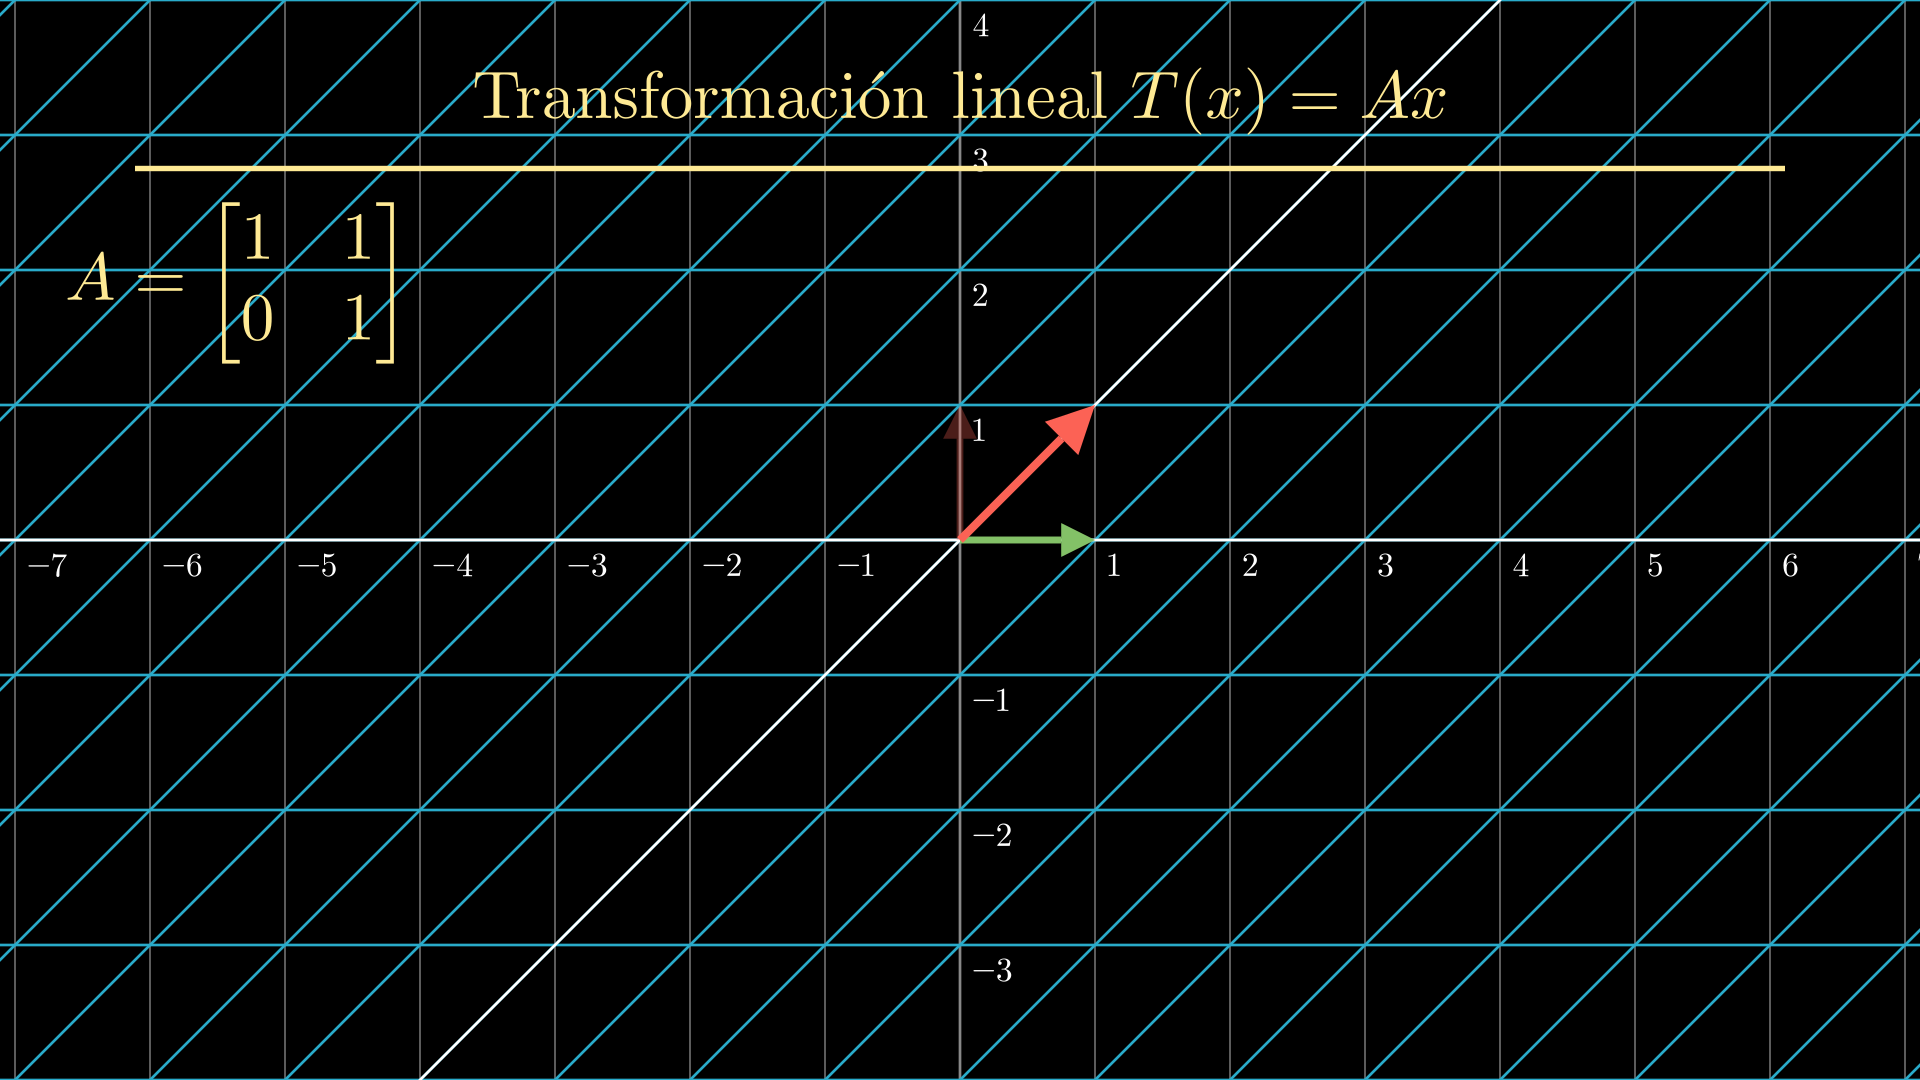
\includegraphics[scale=0.15]{manim/media/images/Transformaciones_lineales/TransformacionLinealEjemplo3_ManimCE_v0.18.0.png}\\
        % \caption{Ejemplo 3}
      \end{center}
    \end{figure}
  \end{center}
\end{frame}

\begin{frame}
  \begin{center}
    \begin{figure}[ht]
      \begin{center}
        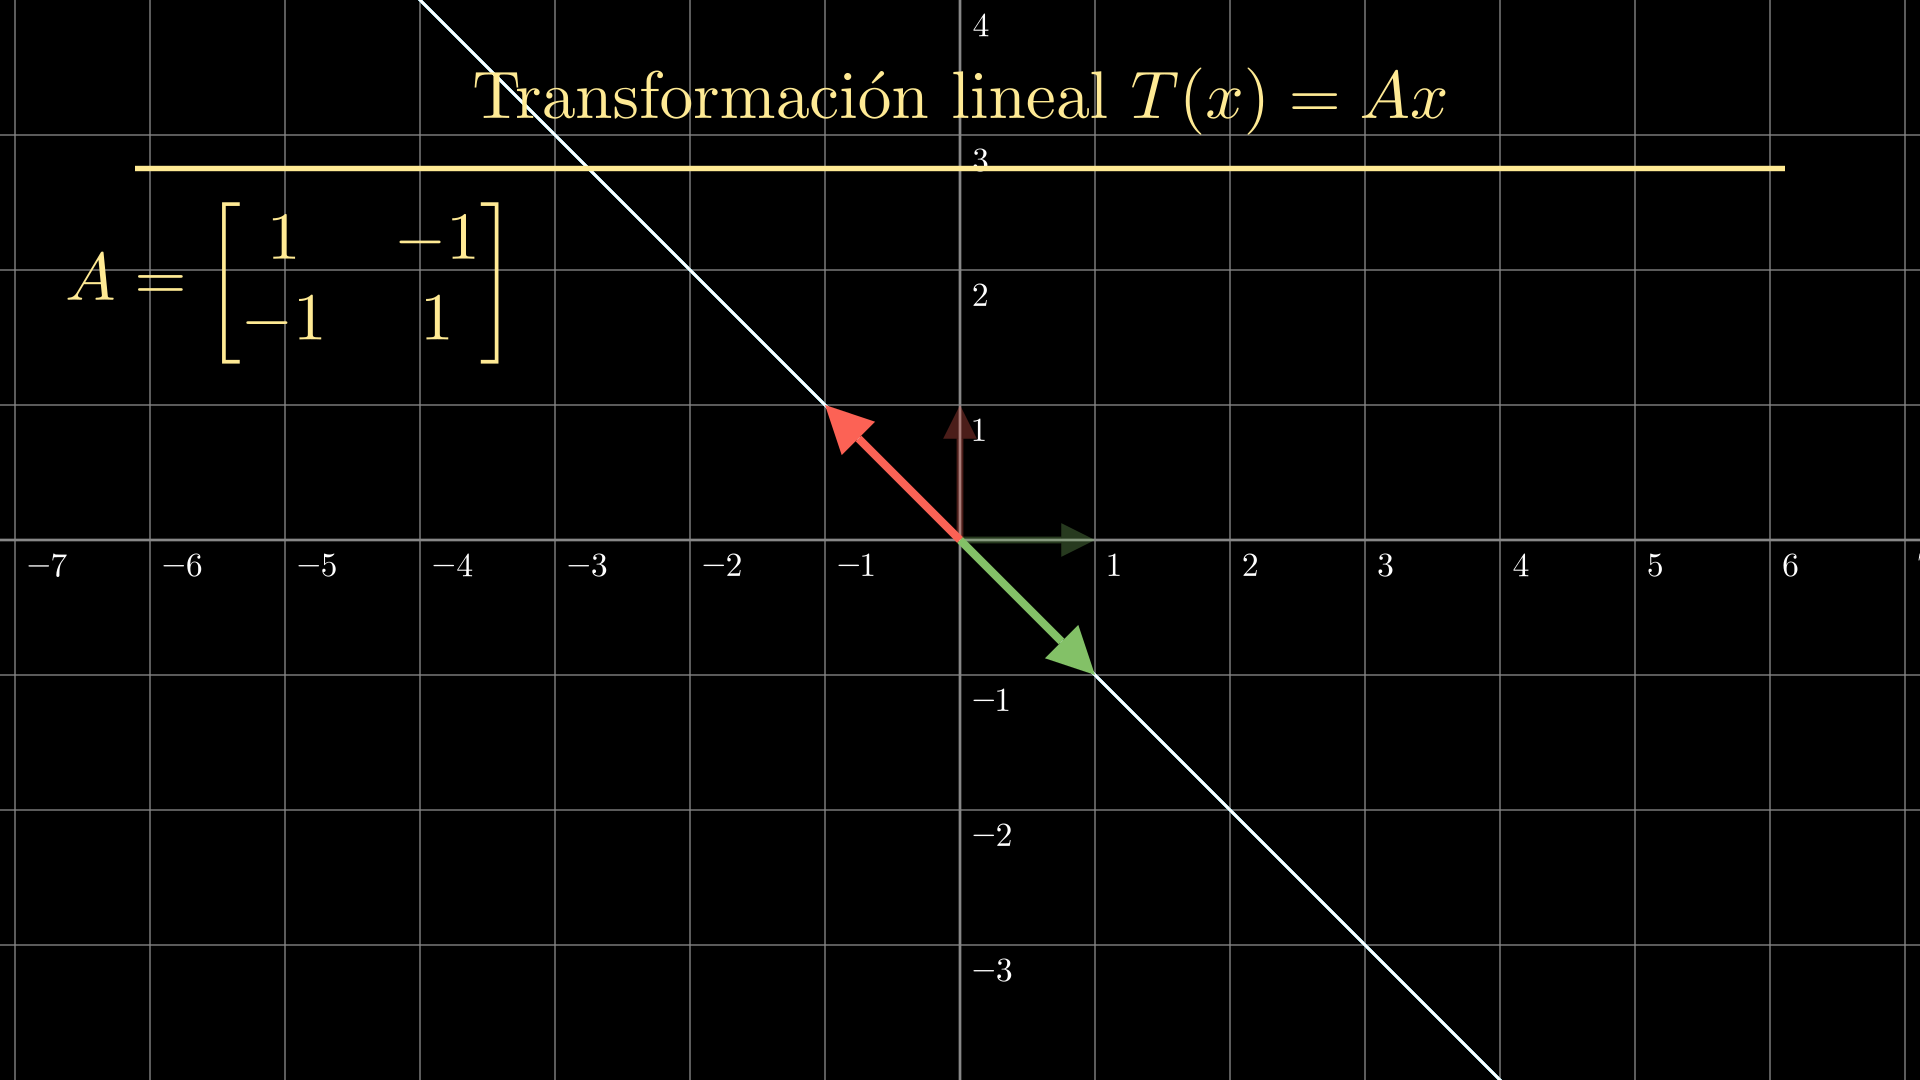
\includegraphics[scale=0.15]{manim/media/images/Transformaciones_lineales/TransformacionLinealEjemplo5_ManimCE_v0.18.0.png}\\
        % \caption{Ejemplo 5}
      \end{center}
    \end{figure}
  \end{center}
\end{frame}


%! subsección
\subsection{Conceptos Básicos de Topología}
\begin{frame}
\subsectionpage
\end{frame}

% \begin{frame}
% \tableofcontents[currentsubsection]
% \end{frame}

\begin{frame}
\begin{defn}
Dados $a\in\Real^n$ y $r>0$, definiremos la \textbf{bola abierta} de centro $a$ y radio $r$, como
$$B(a,r)=\set{\vec{x}\in\Real^n:d(\vec{x},a)<r}$$
% \onslide<2->{
% y \textbf{bola cerrada} de centro $a$ y radio $r$, como
% $$\overline{B(a,r)}=\set{\vec{x}\in\Real^n:d(\vec{x},a)\leq r}$$
% }
\end{defn}
\onslide<2->{
\begin{defn}
Sea $A\subseteq\Real^n$. Diremos que $A$ es \textbf{abierto} si y solo si $$\forall a\in A\exists r>0\ B(a,r)\subseteq A$$
\end{defn}
}
\onslide<3->{
\begin{defn}
Sea $A\subseteq\Real^n$. Diremos que $A$ es \textbf{cerrado} si y solo si $A^c$ es abierto
\end{defn}
}
\end{frame}

\begin{frame}
\begin{defn}
Sea $A\subseteq\Real^n$. Diremos que $a\in\Real^n$ es un \textbf{punto interior} de $A$ si y solo si
$$\exists r>0\ B(a,r)\subseteq A$$
al conjunto de puntos interiores de $A$ lo denotaremos por $\interior{A}$ o $\text{Int}(A)$
\end{defn}
\onslide<2->{
\begin{rem}
    Un conjunto A es abierto si y solo si $\interior{A}=A$
\end{rem}
}
\onslide<3->{
\begin{defn}
Sea $A\subseteq\Real^n$. Diremos que $a\in\Real^n$ es un \textbf{punto exterior} de $A$ si y solo si $a\in\text{Int}(A^c)$
\end{defn}
}
\end{frame}

\begin{frame}
\begin{defn}
  Sea $A\subseteq\Real^n$. Diremos que $a\in\Real^n$ es un \textbf{punto de adherencia} de $A$ si y solo si
  $$\forall r>0\ B(a,r)\cap A\neq\varnothing$$
  al conjunto de puntos de adherencia de $A$ se le conoce como \textbf{Clausura de $A$} y lo denotaremos por $\overline{A}$.
\end{defn}
\onslide<2->{
  \begin{rem}
    Un conjunto A es cerrado si y solo si $\overline{A}=A$
  \end{rem}
}
\end{frame}

\begin{frame}
\begin{defn}
Sea $A\subseteq\Real^n$. Diremos que $a\in\Real^n$ es un \textbf{punto de acumulación} de $A$ si y solo si
$$\forall r>0\ (B(a,r)-\set{a})\cap A\neq\varnothing$$
al conjunto de los puntos de acumulación de $A$ lo llamaremos \textbf{Derivado de $A$} y lo denotaremos como $A'$.
\end{defn}
\onslide<2->{
\begin{defn}
Sea $A\subseteq\Real^n$. Diremos que $a\in\Real^n$ es un \textbf{punto frontera} de $A$ si y solo si
$$\forall r>0\ (B(a,r)\cap A\neq\varnothing)\wedge(B(a,r)\cap A^c\neq\varnothing)$$
al conjunto de puntos frontera de $A$ lo llamaremos \textbf{frontera de $A$} lo denotaremos por $\delta A$ o $\text{Fr}(A)$.
\end{defn}
}
\end{frame}

\begin{frame}
\begin{defn}
  Sea $A\subseteq\Real^n$. Diremos que $A$ es \textbf{acotado} si y solo si 
  $$\exists M>0\ \forall a\in A\ \norm{a}\leq M$$
\end{defn}
\onslide<2->{
\begin{defn}
  Sea $A\subseteq\Real^n$. Diremos que $A$ es \textbf{compacto} si y solo si $A$ es cerrado y acotado.
\end{defn}
}
\end{frame}

\begin{frame}
\begin{defn}
  Sea $A\subseteq\Real^n$. Diremos que $A$ es \textbf{disconexo} si existen abiertos $U$ y $V$ tales que $U\cap V=\varnothing$, $U\cap A\neq\varnothing$, $V\cap A\neq\varnothing$ y $A\subseteq U\cup V$.
\end{defn}
\onslide<2->{
\begin{defn}
  Sea $A\subseteq\Real^n$. Diremos que $A$ es \textbf{conexo} si y solo si $A$ no es disconexo.
\end{defn}
}
\end{frame}

\begin{frame}
\begin{defn}
Sea $A\subseteq\Real^n$, $A\neq\varnothing$. Diremos que $A$ es una \textbf{región} si y solo si $A$ es abierto y conexo
\end{defn}
\end{frame}

\begin{frame}{Ejemplos}
\begin{enumerate}
  \item $\Real^n$ y $\varnothing$ son abiertos y cerrados.
  \item $B(a,r)$ es abierta.
  \item La bola cerrada $B[a,r]=\overline{B(a,r)}$ es cerrada.
  \item El conjunto $\set{(x,y)\in\Real^2:x+2y<1}$ es abierto.
  \item El conjunto $\set{(x,y)\in\Real^2:x+2y\leq1}$ es cerrado.
\end{enumerate}
\end{frame}

%! subsección
\subsection{Ejercicios}
\begin{frame}
\subsectionpage
\end{frame}

% \begin{frame}
% \tableofcontents[currentsubsection]
% \end{frame}

\begin{frame}{Ejercicios}
  Determine cuales de las siguientes funciones son transformaciones lineales
  %\vspace{-0.5cm}
  \begin{enumerate}
  \item $T:\Real^2\To \Real^2$ definida por $$T(x,y)=(5x-2y,y-2x)$$
  %\item $T:\Real_n[x]\To\Real_{n+1}[x]$ definida por $$T(p)=D(p)+I_x(p)$$
  \item $T:\Real^2\To\Real$ tal que $$T(x,y)=x^2-xy$$
  %\item $T:\Real^2\To\Real^3$ tal que $T(x,y)=(x,x-y,xy^2)$
  %\item $T:\Real^n\To\Real^n$ definida por $T(u)=Au+u_0$, donde $A\in\mathcal{M}_{m\times n}(\Real)$ y $u_0\in\Real^m$ están fijos.
  \item $T:\Real^2\To \Real^2$ definida por $$T(x,y)=(3x+y-1,y-x+2)$$
  \end{enumerate}
\end{frame}

\begin{frame}{Ejercicios}
  \begin{enumerate}
  \setcounter{enumi}{3}
  \item  Sea $T:\Real^2\to\Real^3$ una transformación lineal tal que.
  $$T(1,0)=(1,1,2),\ \ T(0,1)=(1,1,-1)$$
  Determine $T(x,y)$ y su matriz canónica, $\forall(x,y)\in\Real^2$.
  \vspace{5mm}
  \item  Sea $T:\Real^3\to\Real^3$ una transformación lineal tal que.
  $$T(1,0,0)=(2,0,3),\ T(0,1,0)=(-1,1,1),\ T(0,0,1)=(1,1,4)$$
  Determine $T(x,y,z)$ y su matriz canónica, $\forall(x,y,z)\in\Real^3$.
  %\item  Sea $T:\Real_2[x]\to\mathcal{M}_{2\times3}(\Real)$ una transformación lineal tal que.
  %$$T(1+x)=
  %\left[\begin{array}{rrr}
  %2 & 3 & 4\\
  %6 & 7 & 8
  %\end{array}\right],\ 
  %T(1+x^2)=
  %\left[\begin{array}{rrr}
  %2 & 3 & 4\\
  %0 & 0 & 0
  %\end{array}\right],\ 
  %T(x+x^2)=
  %\left[\begin{array}{rrr}
  %0 & 0 & 0\\
  %6 & 7 & 8
  %\end{array}\right]
  %$$
  %Determine $T(a+bx+cx^2)$, $\forall a+bx+cx^2\in\Real_2[x]$.
  \end{enumerate}
\end{frame}

\begin{frame}
  \begin{enumerate}
  \setcounter{enumi}{5}
  \item En los siguientes conjuntos, grafique el conjunto y determine si son abiertos, cerrados, compactos, conexos, disconexos, regiones o ninguno de los anteriores.
    \vspace{6mm}
    \begin{enumerate}
      \item $\set{(x,y)\in\Real^2\ :\ x^2+y^2 \leq 1\wedge y>x}$
      \vspace{2mm}
      \item $\set{(x,y)\in\Real^2\ :\ x<1-y^2 \wedge x+y+1> 0}$
      \vspace{2mm}
      \item $\set{(x,y)\in\Real^2\ :\ x^2+2y^2\leq 4 \wedge y-x^2\geq 0}$
      \vspace{2mm}
      \item $\set{(x,y)\in\Real^2\ :\ x^2+y^2<2x\wedge x\leq y}$
      \vspace{2mm}
      \item $\set{(x,y)\in\Real^2\ :\ 4x^2+9y^2\leq 36\wedge \abs{x}\geq 1}$
      \vspace{2mm}
      \item $\set{(x,y)\in\Real^2\ :\ 2x+y>2\wedge x^2-y<0}$
    \end{enumerate}
  \end{enumerate}
\end{frame}


%! sección
\section{Funciones de Varias Variables}
\begin{frame}
\sectionpage
\end{frame}

\begin{frame}
\tableofcontents[currentsection]
\end{frame}

%! subsección
\subsection{Funciones de Varias Variables}
\begin{frame}
\subsectionpage
\end{frame}

% \begin{frame}
% \tableofcontents[currentsubsection]
% \end{frame}

\begin{frame}
\vspace{-0.5cm}
\begin{defn}
  \begin{itemize}[<+->]
    \item Llamaremos \textbf{función real de varias variables}, \textbf{función escalar} o \textbf{campo escalar} de varias variables a las funciones del tipo 
    $$f:A\subseteq\Real^n\to\Real$$
    \item Llamaremos \textbf{función vectorial} a las funciones del tipo 
    $$f:A\subseteq\Real^n\to\Real^m$$
    \item Llamaremos \textbf{Curva} o \textbf{trayectoria} a las funciones del tipo
    $$f:A\subseteq\Real\to\Real^n$$
    En este caso usualmente $A=[a,b]$, con $a,b\in\Real$.
  \end{itemize}
\end{defn}
\vspace{-0.25cm}
\onslide<4->{
  \begin{rem}
    Una función $f:\Real^n\to\Real^n$, $n\geq 2$, también es llamada \textbf{campo vectorial}.
  \end{rem}
}
\end{frame}

\begin{frame}{Ejemplos}
\begin{enumerate}
  \item $f(x,y)=x^2+y^2$ es una función real de varias variables.
  \item $f(x,y)=(x^2+y^2,x^2-y^2)$ es una función vectorial de varias variables.
  \item $f(t)=(\cos(t),\sen(t))$ es una curva.
\end{enumerate}
\end{frame}

\begin{frame}
  \begin{defn}
    Sea $f:A\subseteq\Real^n\to\Real^m$.
    \begin{itemize}[<+->]
      \item El dominio de $f$ debiese ser $A$ y lo denotaremos $A=\text{Dom}(f)$.\\[0.25cm]
      \item El recorrido de $f$ es el conjunto
      $$\text{Rec}(f)=\set{y\in\Real^m\ :\ \exists x\in A\ y=f(x)}$$
    \end{itemize}
  \end{defn}
\end{frame}

\begin{frame}{Ejemplos}
  \begin{enumerate}
    \item Encuentre el recorrido de $f(x,y)=x^2+y^2$.
    \item Encuentre el dominio de $f(x,y)=\sqrt{1-x^2-y^2}$.
  \end{enumerate}
\end{frame}

\begin{frame}
  \begin{thm}
    Sea $f:A\subseteq\Real^n\to\Real^m$. Entonces existen funciones escalares $f_1, f_2, \ldots, f_m:A\subseteq\Real^n\to\Real$ tales que $f(x)=(f_1(x),f_2(x)\ldots,f_m(x))$.
  \end{thm}
  \onslide<2->{
    \begin{rem}
      Llamaremos \textbf{componentes} a las funciones $f_1, f_2, \ldots, f_m$ y anotaremos $f=(f_1,f_2,\ldots,f_m)$.
    \end{rem}
  }
\end{frame}

\begin{frame}
\begin{defn} 
  Sea $f:A\subseteq\Real^n\to\Real$, Definimos el \textbf{gráfico} de $f$ como
  $$Gr(f)=\set{(x_1,x_2,\ldots,x_n,x_{n+1})\in\Real^{n+1}:x_{n+1}=f(x_1,x_2,\ldots,x_n)}$$
\end{defn}
\onslide<2->{
\begin{rem}
  El gráfico definido de esta manera es una forma de representar la función escalar $f$ en $\Real^{n+1}$. En el caso $n=1$ el gráfico es una curva en el plano, en el caso $n=2$ el gráfico es una superficie en el espacio.\\
  \vspace{2mm}
\onslide<3->{
  \par Las siguientes figuras muestran esta y otras formas de representar gráficamente funciones de varias variables y funciones vectoriales.
}
\end{rem}
}
\end{frame}

\begin{frame}{Gráfico de una función real de dos variables}
  \begin{figure}
    \begin{center}
      
\includegraphics[scale=0.5]{./Imagenes/Funcion3D.png}
      \caption{$f(x,y)=\sen(\sqrt{x^2+y^2})$}
    \end{center}
  \end{figure}
\end{frame}

\begin{frame}{Gráfico de un Campo Escalar}
  \begin{figure}
    \begin{center}
      
\includegraphics[scale=0.5]{./Imagenes/Campo_Escalar.png}
      \caption{$f(x,y)=\sen(x^2+y^2)$}
    \end{center}
  \end{figure}
\end{frame}

\begin{frame}{Gráfico de un Campo Vectorial}
  \begin{figure}
    \begin{center}
      
\includegraphics[scale=0.5]{./Imagenes/Campo_de_vectores.png}
      \caption{$f(x,y)=(x^2+y^2,x^2-y^2)$}
    \end{center}
  \end{figure}
\end{frame}

% gráficos de funciones vectoriales de MAT014

\begin{frame}{Gráfico de un Campo Vectorial}
  \begin{figure}
    \begin{center}
      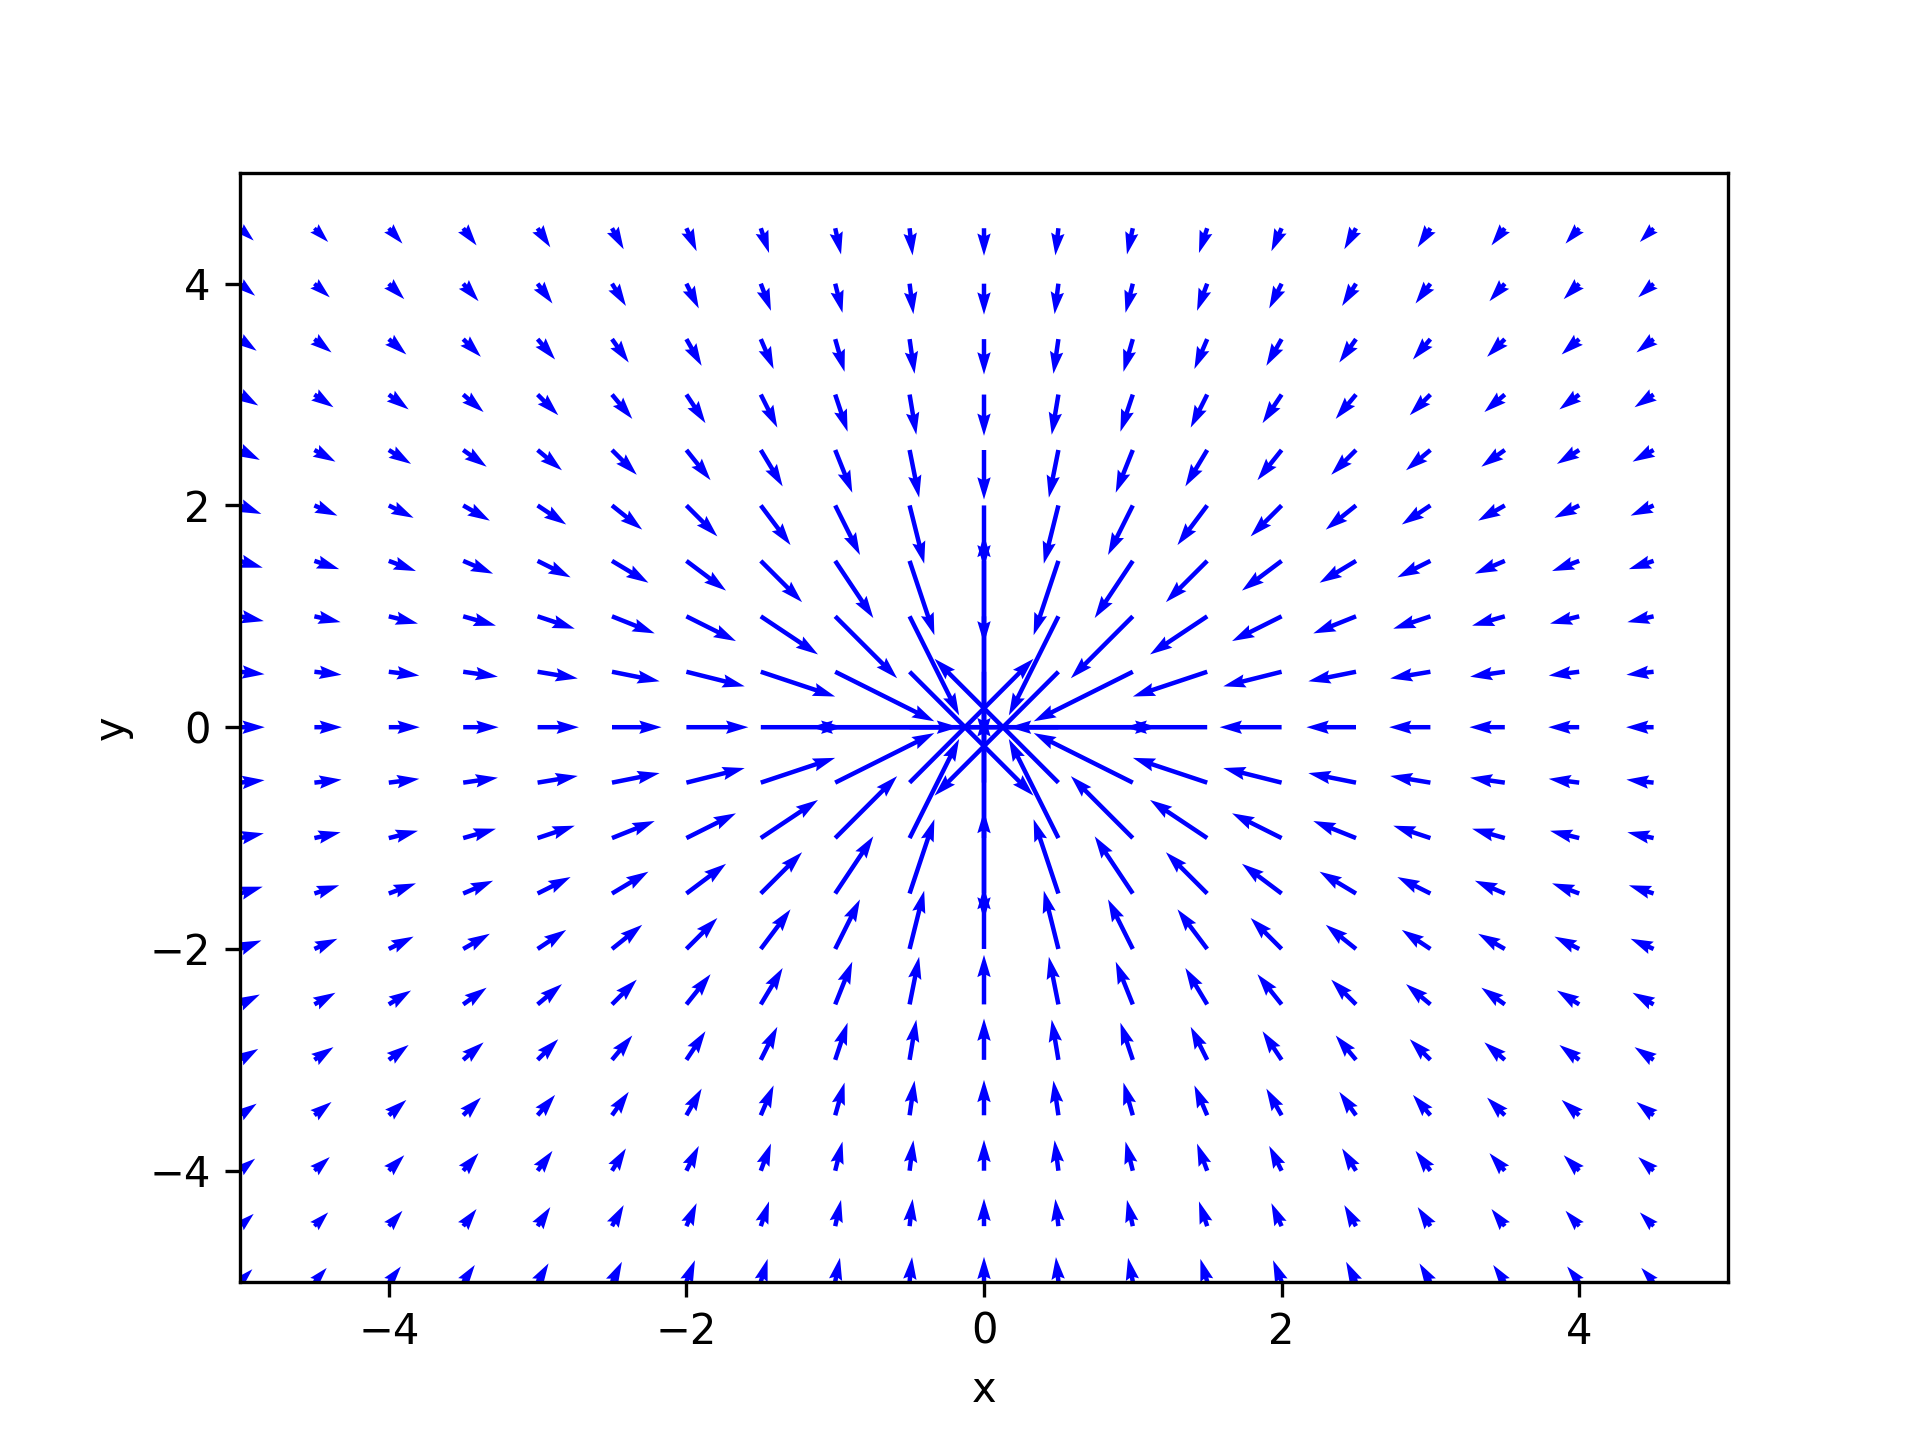
\includegraphics[scale=0.5]{./imagenes/Campo_de_Vectores_feo.png}
      \caption{$f(x,y)=\left(\dfrac{-x}{x^2+y^2},\dfrac{-y}{x^2+y^2}\right)$}
    \end{center}
  \end{figure}
\end{frame}

\begin{frame}{Gráfico de un Campo Vectorial}
  \begin{figure}[ht]
    \begin{center}
      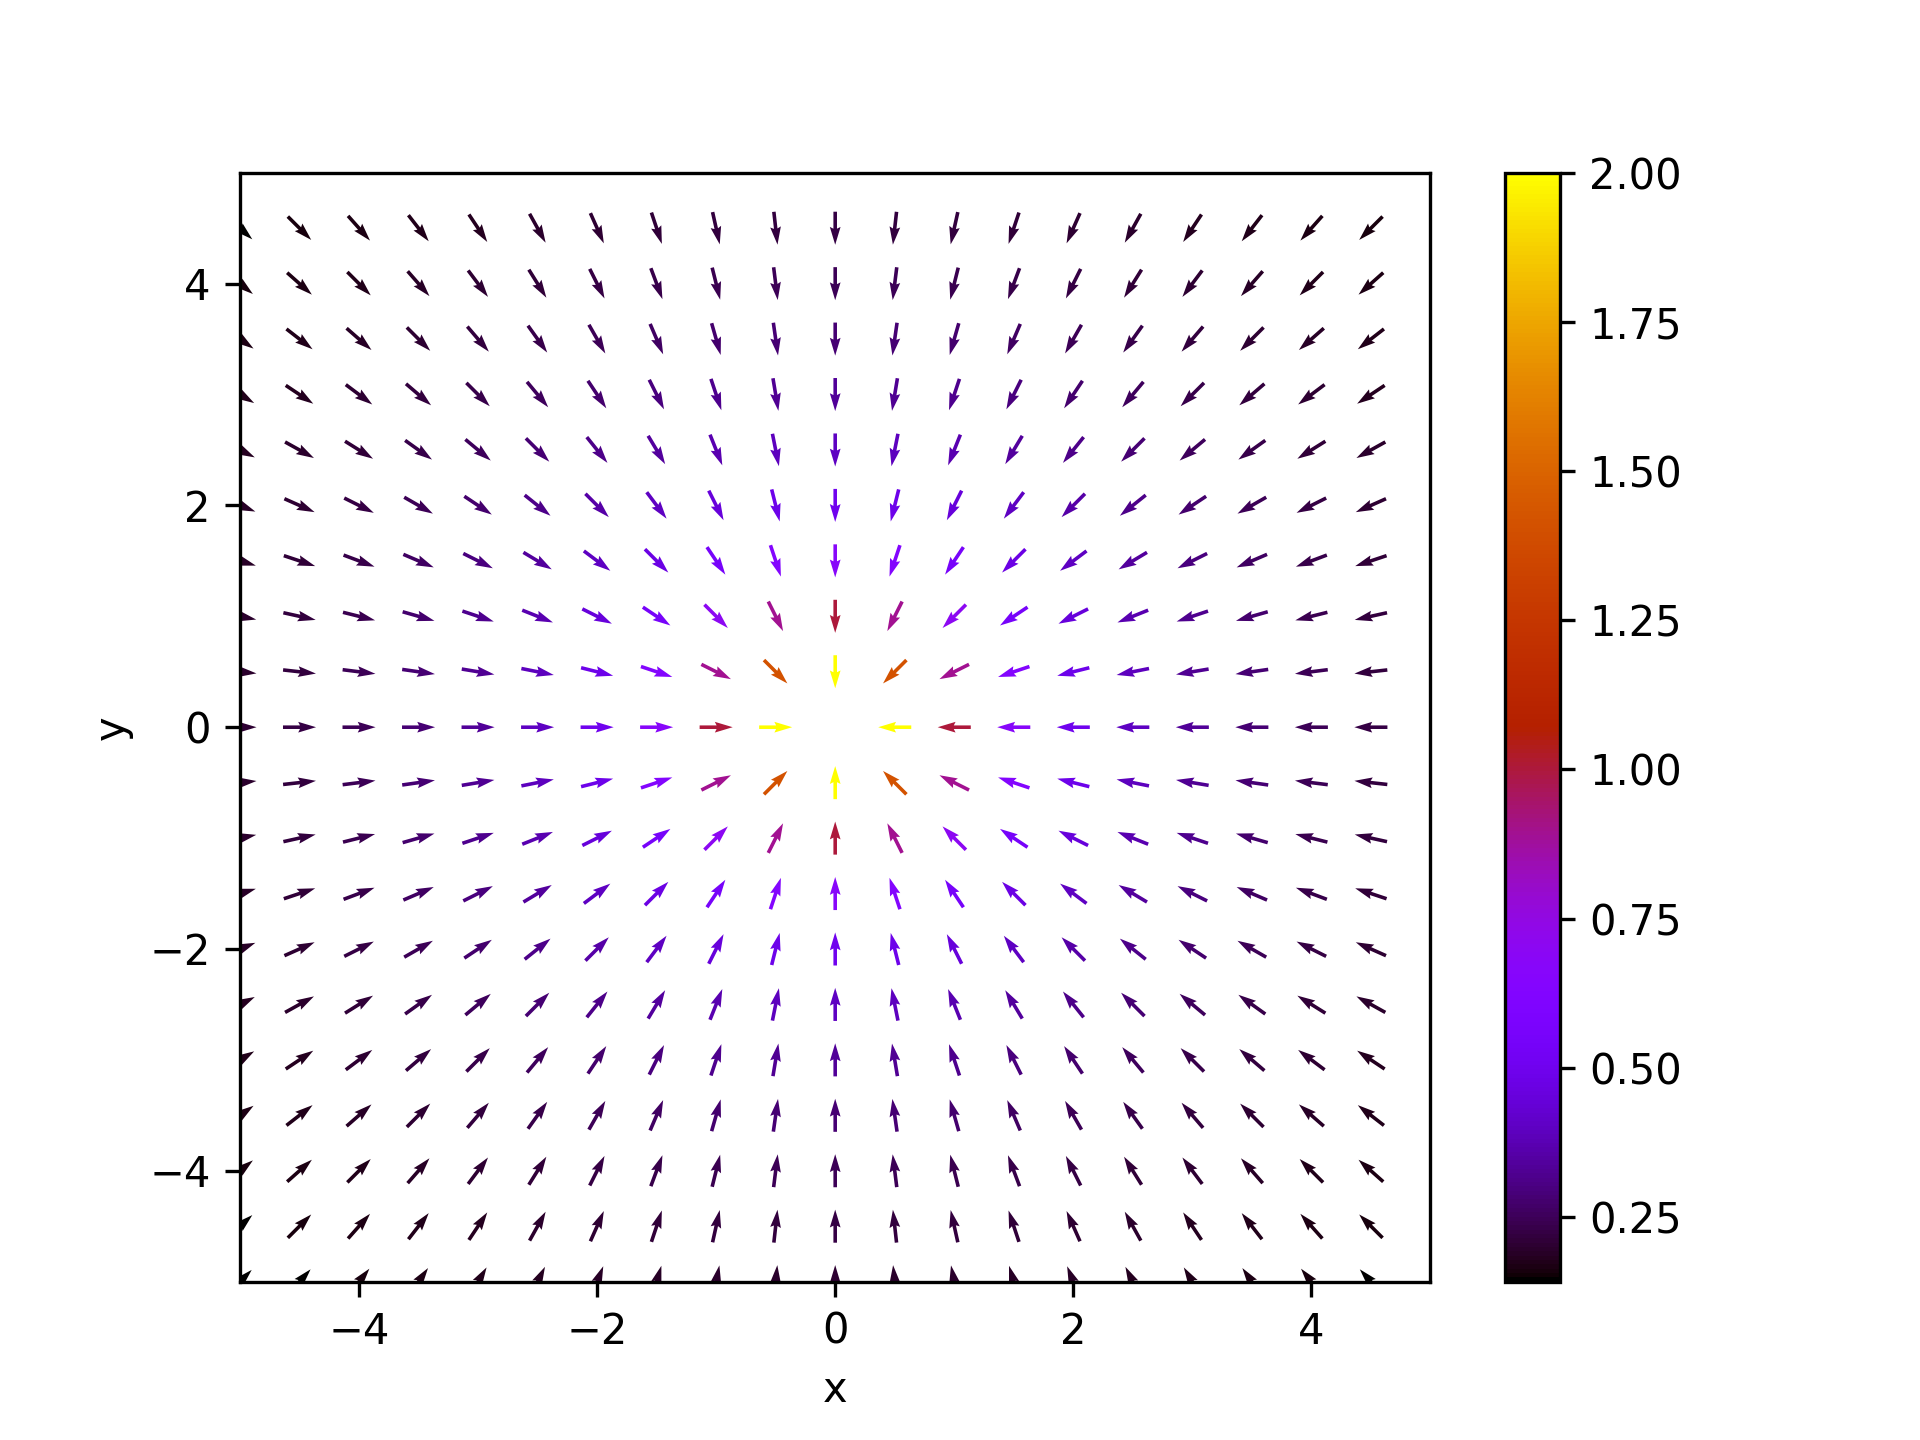
\includegraphics[scale=0.5]{./imagenes/Campo_de_Vectores_norm_color.png}
      \caption{$f(x,y)=\left(\dfrac{-x}{x^2+y^2},\dfrac{-y}{x^2+y^2}\right)$}
    \end{center}
  \end{figure}
\end{frame}

\begin{frame}{Gráfico de un Campo Vectorial en el Espacio}
  \vspace{-1cm}
  \begin{figure}
    \begin{center}
      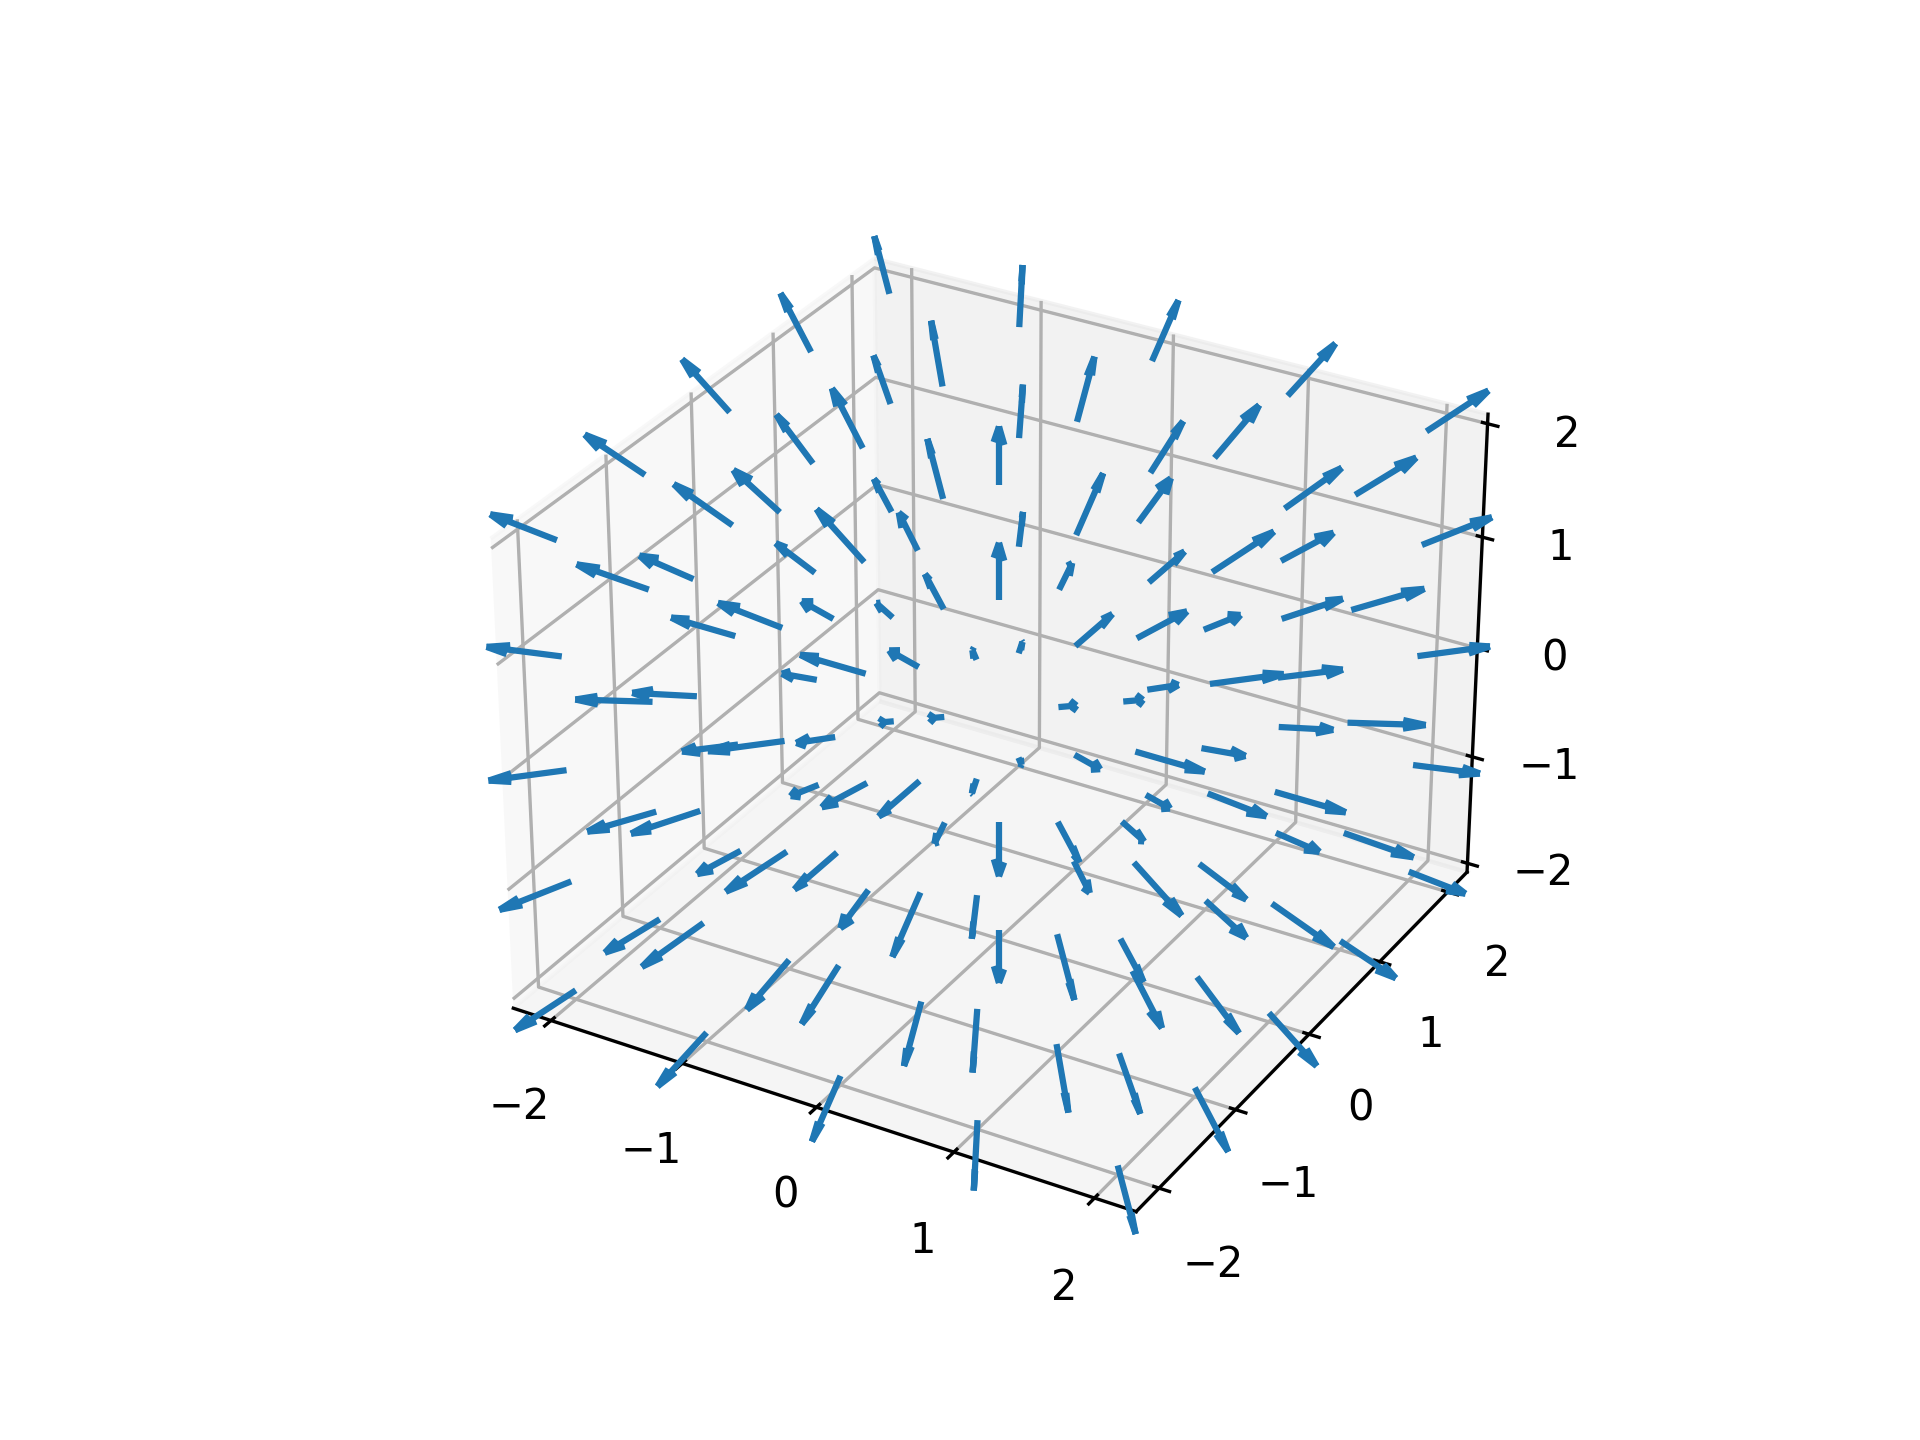
\includegraphics[scale=0.6]{./imagenes/Campo_de_vectores_3D.png}
      \caption{$f(x,y,z)=\left(x,y,z\right)$}
    \end{center}
  \end{figure}
\end{frame}

\begin{frame}{Gráfico de una Curva en el Plano}
  \begin{figure}
    \begin{center}
      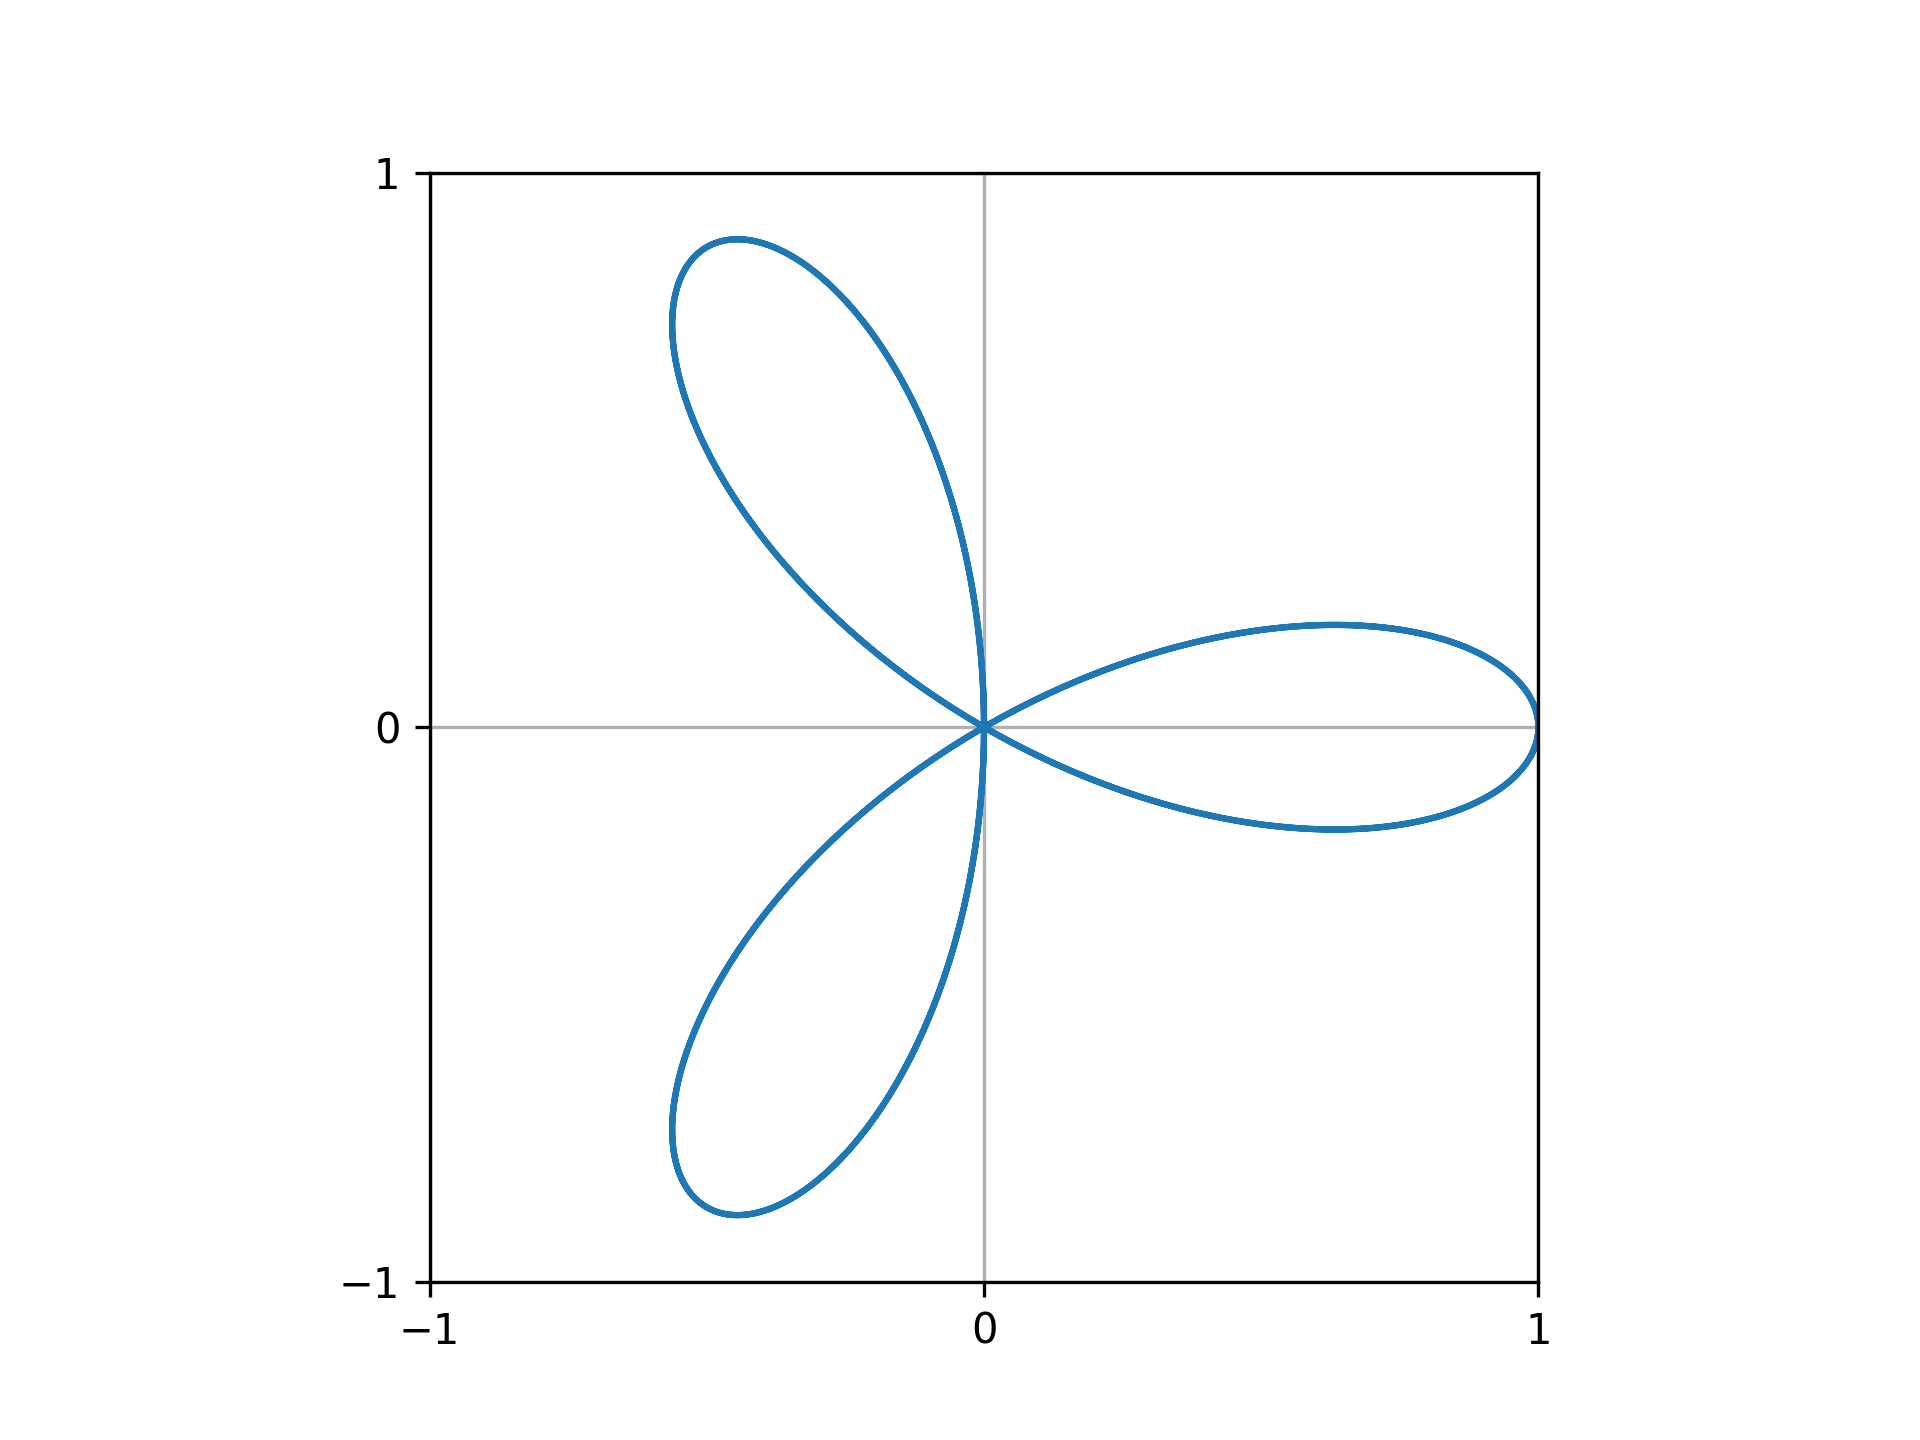
\includegraphics[scale=0.5]{./imagenes/Curva_parametrica_2D.png}
      \caption{$f(t)=(\cos(3t)\cos(t),\cos(3t)\sen(t))$}
    \end{center}
  \end{figure}
\end{frame}

\begin{frame}{Gráfico de una Curva en el Espacio}
  \vspace{-1cm}
  \begin{figure}
    \begin{center}
      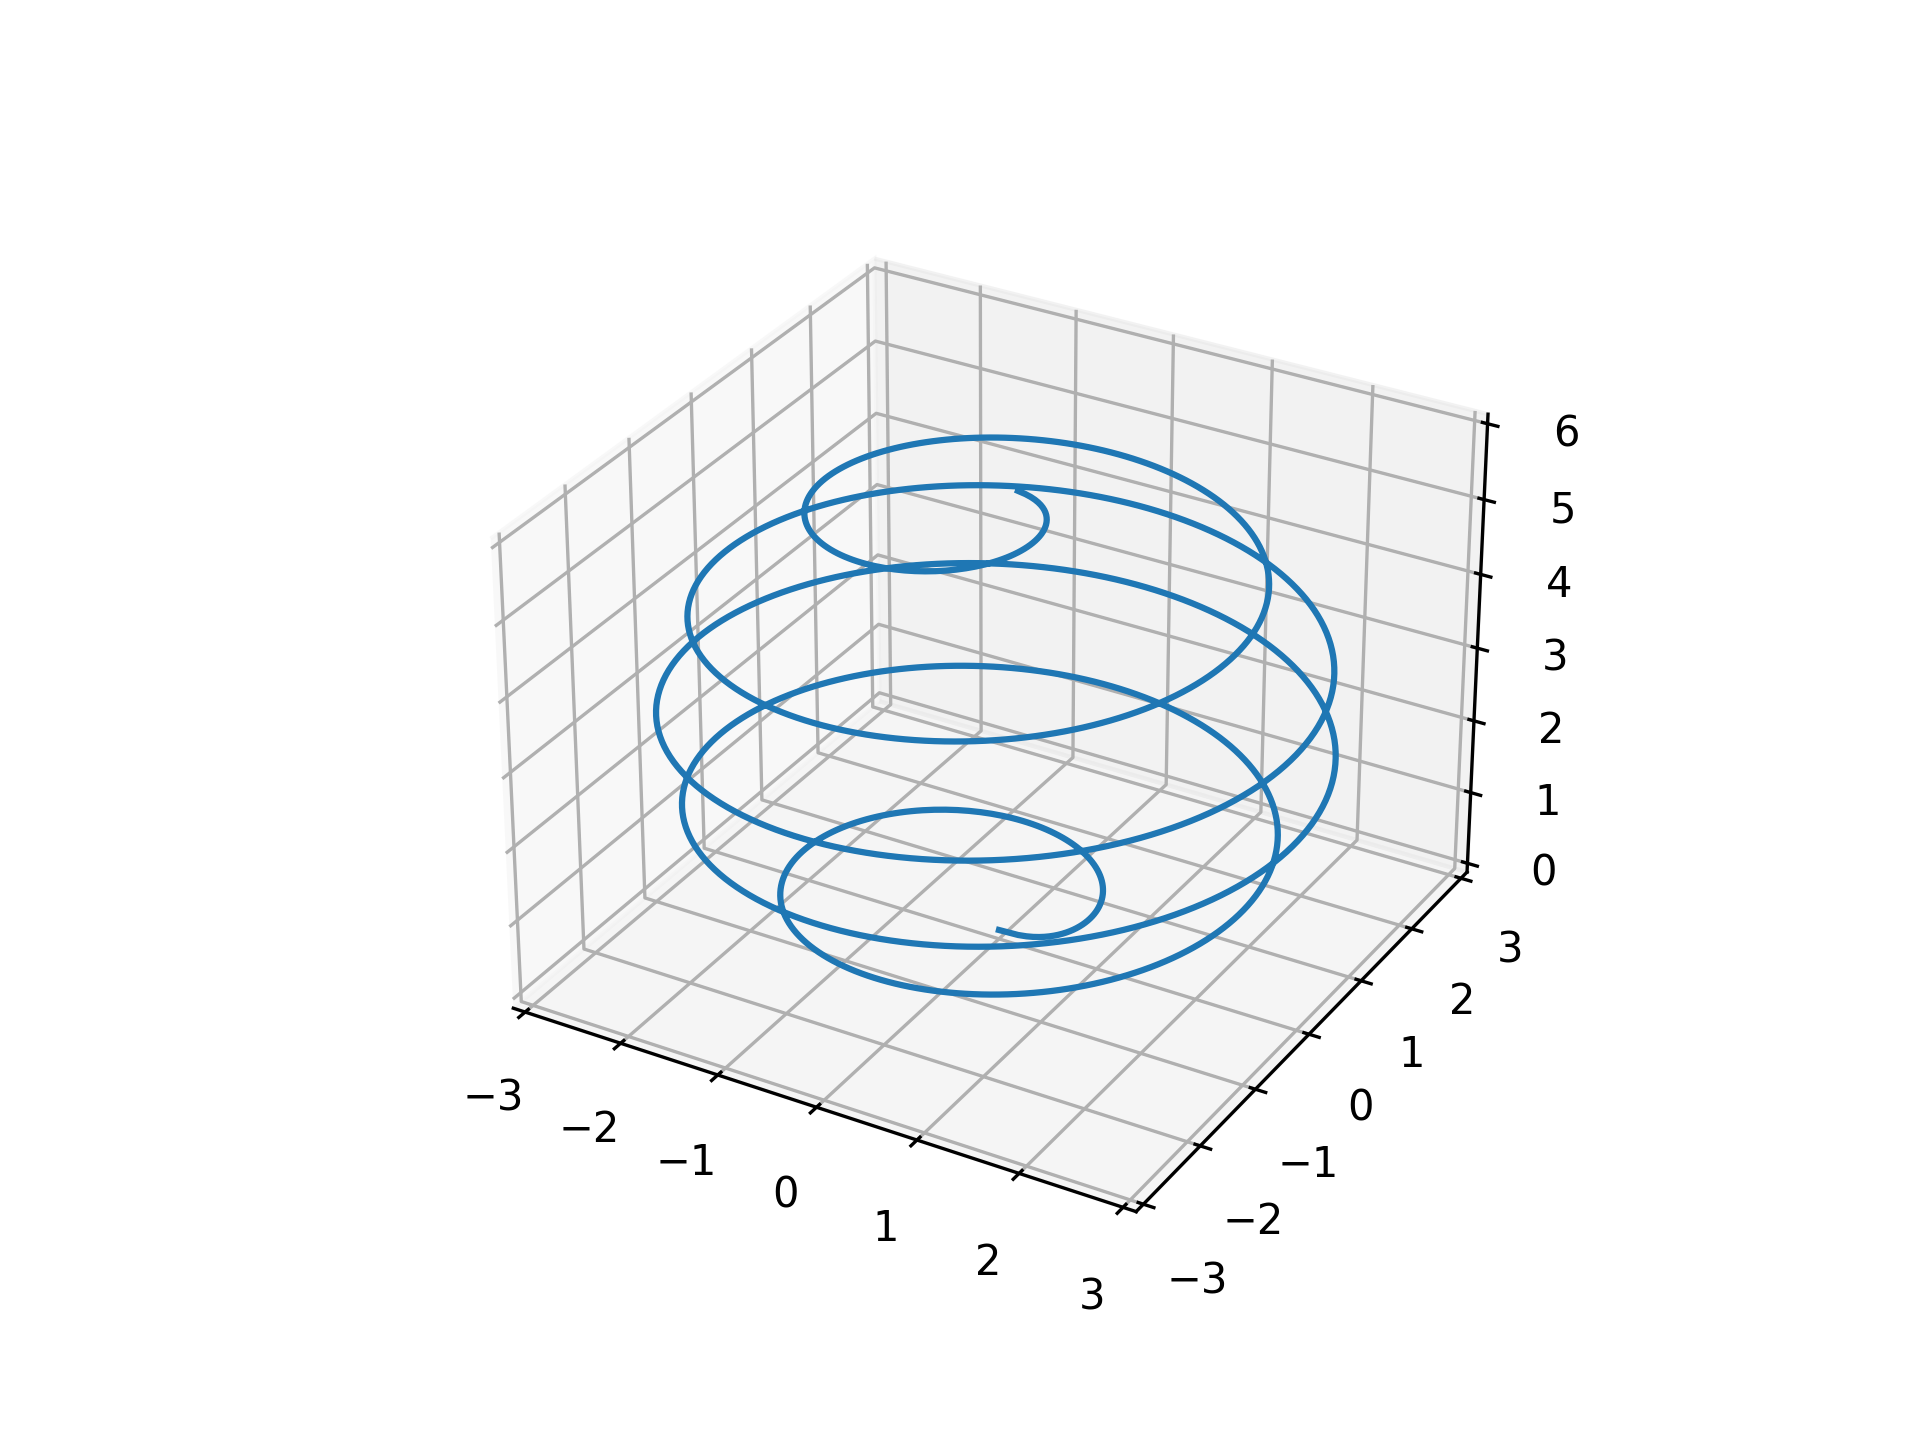
\includegraphics[scale=0.6]{./imagenes/Curva_parametrica_3D.png}
      \caption{$f(t)=(\sqrt{9-(t-3)^2}\cos(10\pi t/6),\sqrt{9-(t-3)^2}\sen(10\pi t/6),t)$}
    \end{center}
  \end{figure}
\end{frame}

\begin{frame}{Grafico de una Superficie Paramétrica}
  \vspace{-1cm}
  \begin{figure}
    \begin{center}
      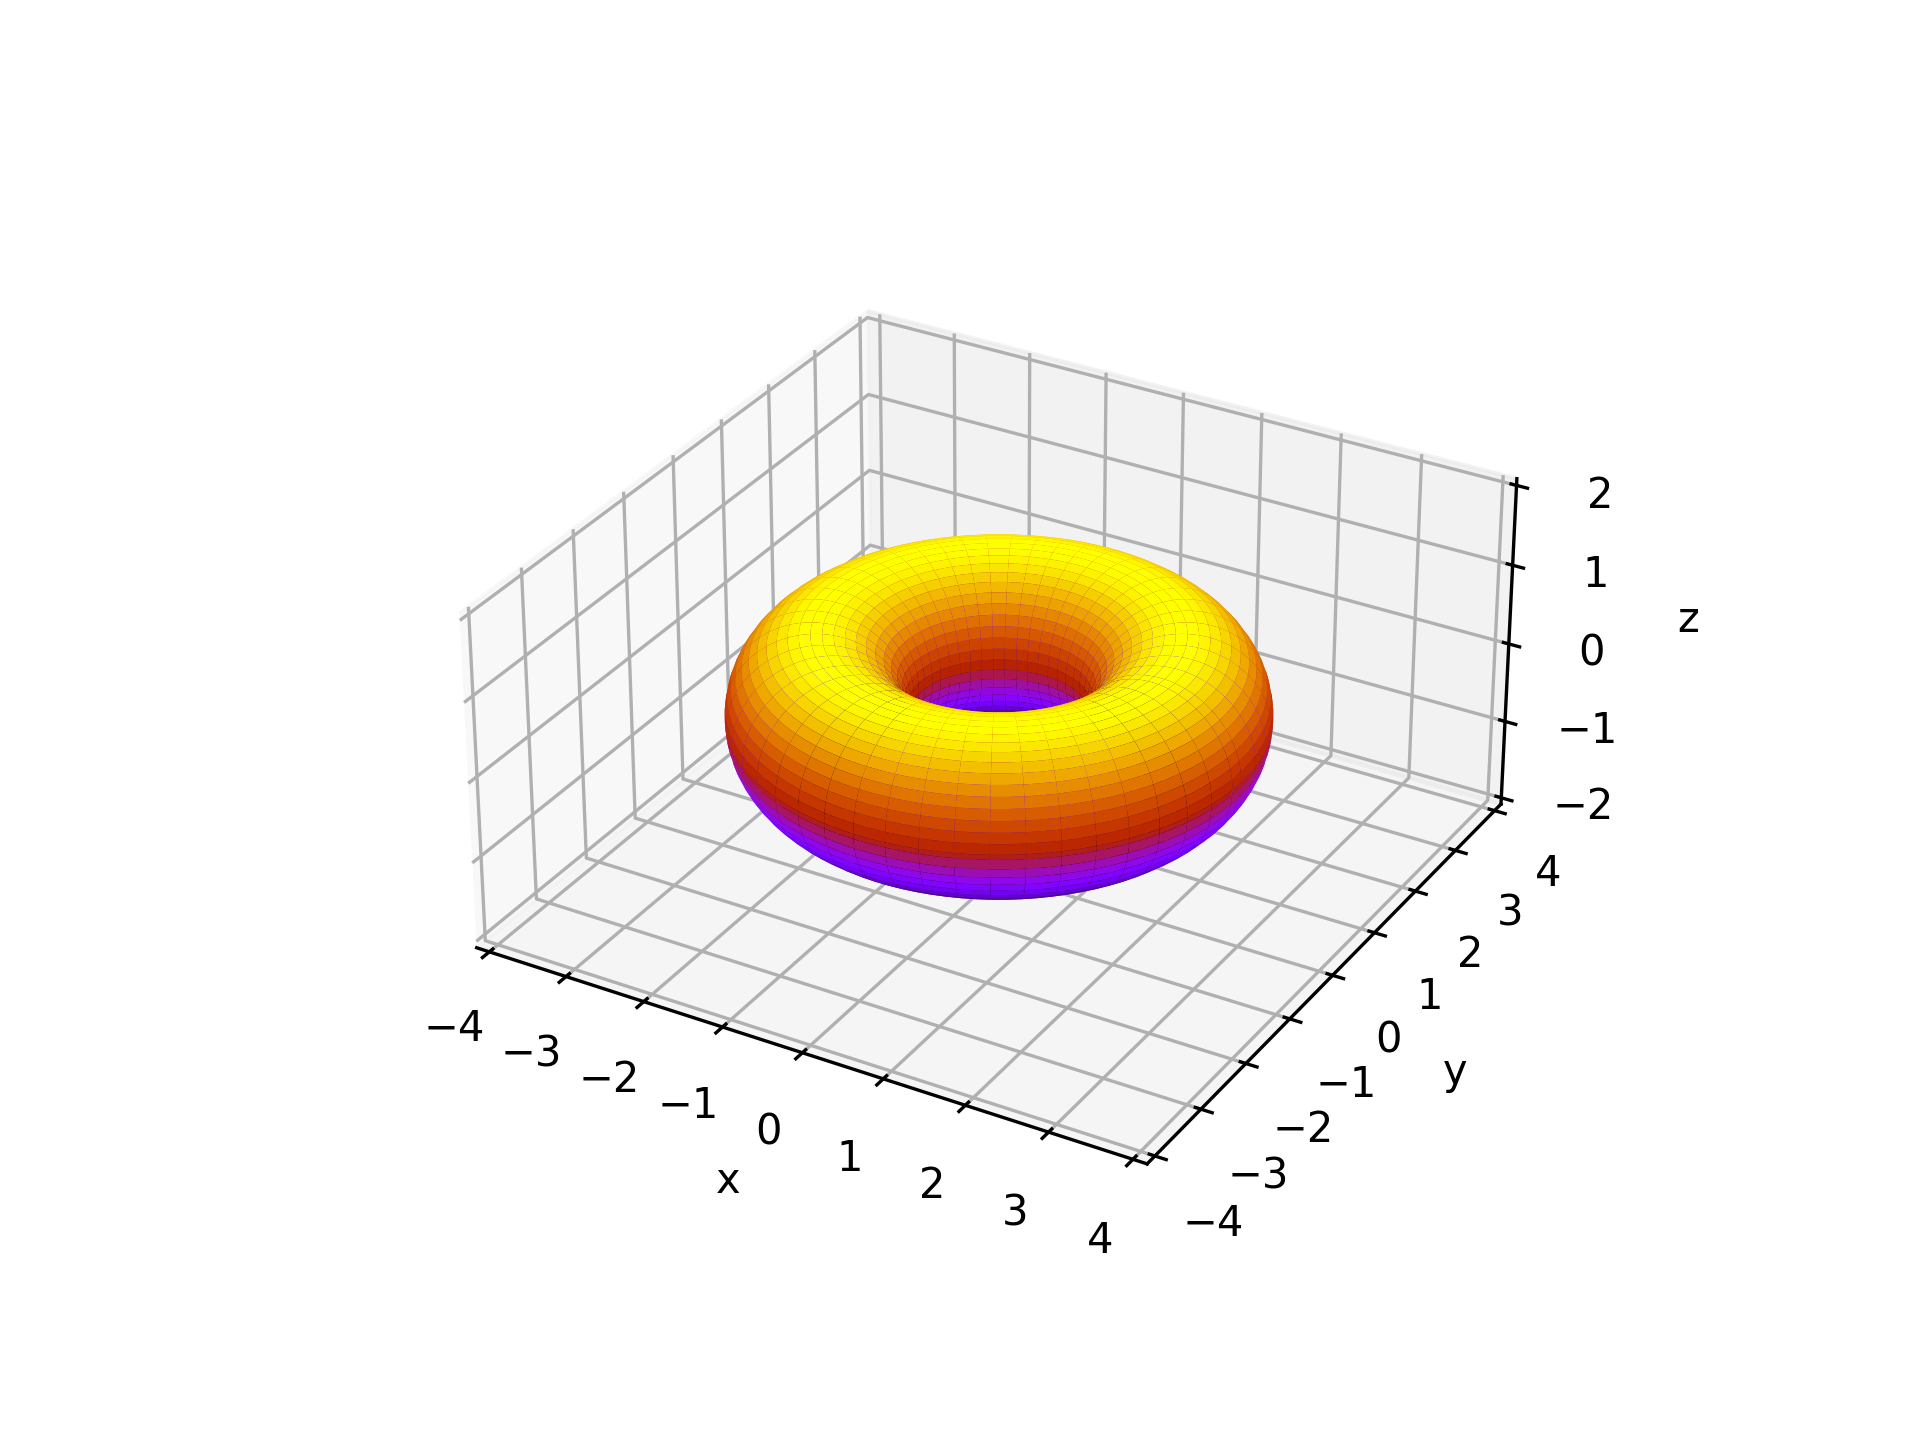
\includegraphics[scale=0.6]{./imagenes/Toro_parametrico.png}
      \caption{$f(u,v)=((2+\cos(v))\cos(u),(2+\cos(v))\sen(u),\sen(v))$}
    \end{center}
  \end{figure}
\end{frame}

% fin gráficos de funciones vectoriales de MAT014

\begin{frame}
\begin{defn}
Sea $f:A\subseteq\Real^2\to\Real$. Para cada $z_0\in\text{Rec}(f)$ definimos la  correspondiente \textbf{curva de nivel} como el conjunto
$$C_{z_0}=\set{(x,y)\in A:f(x,y)=z_0}$$
\end{defn}
\onslide<2->{
\begin{defn}
Sea $f:A\subseteq\Real^3\to\Real$. Para cada $w_0\in\text{Rec}(f)$ definimos la  correspondiente \textbf{superficie de nivel} como el conjunto
$$S_{w_0}=\set{(x,y,z)\in A:f(x,y,z)=w_0}$$
\end{defn}
}
\onslide<3->{
\begin{rem}
  Las curvas de nivel y superficies de nivel se pueden usar para entender el comportamiento de estas funciones.\\
\vspace{2mm}
\onslide<4->{
  \par Las siguientes figuras muestran como se pueden usar las curvas de nivel para entender el comportamiento de una función real de dos variables.
}
\end{rem}
}
\end{frame}


\begin{frame}{Curvas de nivel de una función real de dos variables}
  \begin{figure}
    \begin{center}
      
\includegraphics[scale=0.5]{./Imagenes/Curvas_de_nivel.png}
      \caption{$f(x,y)=\sqrt{x^2+y^2}$}
    \end{center}
  \end{figure}
\end{frame}

\begin{frame}{Curvas de nivel puestas en $\Real^3$}
  \begin{figure}
    \begin{center}
      
\includegraphics[scale=0.5]{./Imagenes/Curvas_de_nivel_3D.png}
      \caption{$f(x,y)=\sqrt{x^2+y^2}$}
    \end{center}
  \end{figure}
\end{frame}

\begin{frame}{Gráfico en $\Real^3$}
  \begin{figure}
    \begin{center}
      
\includegraphics[scale=0.5]{./Imagenes/Funcion3D_2.png}
      \caption{$f(x,y)=\sqrt{x^2+y^2}$}
    \end{center}
  \end{figure}
\end{frame}

\subsection{Cuádricas}
\begin{frame}
\subsectionpage
\end{frame}

\begin{frame}{Esfera}
La superficie de ecuación,
$$x^2+y^2+z^2=r^2$$
corresponde a la superficie esfera de centro $(0,0,0)$ y radio $r$
\onslide<2->{
\begin{figure}
\begin{center}

\includegraphics[scale=0.38]{./Imagenes/Esfera.png}
\caption{Esfera}
\end{center}
\end{figure}
}
\end{frame}

\begin{frame}{Elipsoide}
La superficie de ecuación
$$\frac{x^2}{a^2}+\frac{y^2}{b^2}+\frac{z^2}{c^2}=1$$
corresponde a un elipsoide centrado en el origen
\onslide<2->{
\vspace{-5mm}
\begin{figure}
\begin{center}

\includegraphics[scale=0.38]{./Imagenes/Elipsoide.png}
\caption{Elipsoide}
\end{center}
\end{figure}
}
\end{frame}

\begin{frame}{Hiperboloide de Una Hoja}
La superficie de ecuación
$$\frac{x^2}{a^2}+\frac{y^2}{b^2}-\frac{z^2}{c^2}=1$$
corresponde a un hiperboloide de una hoja centrado en el origen
\onslide<2->{
\vspace{-5mm}
\begin{figure}
\begin{center}

\includegraphics[scale=0.38]{./Imagenes/Hiperboloide1.png}
\caption{Hiperboloide de una hoja}
\end{center}
\end{figure}
}
\end{frame}

\begin{frame}{Hiperboloide de Dos Hojas}
La superficie de ecuación
$$\frac{x^2}{a^2}-\frac{y^2}{b^2}-\frac{z^2}{c^2}=1$$
corresponde a un hiperboloide de dos hojas centrado en el origen
\onslide<2->{
\vspace{-5mm}
\begin{figure}
\begin{center}

\includegraphics[scale=0.38]{./Imagenes/Hiperboloide2.png}
\caption{Hiperboloide de dos hojas}
\end{center}
\end{figure}
}
\end{frame}

\begin{frame}{Paraboloide Elíptico}
La superficie de ecuación
$$\frac{x^2}{a^2}+\frac{y^2}{b^2}=cz$$
corresponde a un paraboloide elíptico
\onslide<2->{
\vspace{-5mm}
\begin{figure}
\begin{center}

\includegraphics[scale=0.38]{./Imagenes/Paraboloide1.png}
\caption{Paraboloide elíptico}
\end{center}
\end{figure}
}
\end{frame}

\begin{frame}{Paraboloide hiperbólico}
La superficie de ecuación
$$\frac{x^2}{a^2}-\frac{y^2}{b^2}=cz$$
corresponde a un paraboloide hiperbólico
\onslide<2->{
\vspace{-5mm}
\begin{figure}
\begin{center}

\includegraphics[scale=0.38]{./Imagenes/Paraboloide2.png}
\caption{Paraboloide hiperbólico}
\end{center}
\end{figure}
}
\end{frame}

\begin{frame}{Cono}
La superficie de ecuación
$$\frac{x^2}{a^2}+\frac{y^2}{b^2}=\frac{z^2}{c^2}$$
corresponde a un Cono
\onslide<2->{
\vspace{-5mm}
\begin{figure}
\begin{center}

\includegraphics[scale=0.38]{./Imagenes/Cono.png}
\caption{Cono}
\end{center}
\end{figure}
}
\end{frame}

%! subsección
\subsection{Ejercicios}
\begin{frame}
\subsectionpage
\end{frame}

% \begin{frame}
% \tableofcontents[currentsubsection]
% \end{frame}

\begin{frame}{Ejercicios}
  \begin{enumerate}
    \item Usando curvas de nivel $z=k$ haga un bosquejo de las siguientes superficies\\[0.25cm]
      \begin{enumerate}
        \item $f(x,y)=xy$\\
        \item $f(x,y)=x^2-y^2$\\
        \item $f(x,y)=x^2+9y^2$\\
        \item $f(x,y)=e^{\sqrt{x^2+y^2}}$\\
        \item $f(x,y)=\ln(\sqrt{x^2+y^2})$
      \end{enumerate}
  \end{enumerate}
\end{frame}

\begin{frame}{Ejercicios}
  \begin{enumerate}
    \setcounter{enumi}{1}
    \item Usando curvas de nivel para $x=k$, $y=k$ y $z=k$. Haga un bosquejo de las siguientes superficies Cuádricas\\[0.25cm]
      \begin{enumerate}
        \item $4x^2+9y^2+36z^2=36$
        \item $z=x^2-y^2$
        \item $-x^2+4y^2-z^2=4$
      \end{enumerate}
    \vspace{0.5cm}
    \item Escriba las siguientes ecuaciones en forma estándar y realice un bosquejo de la superficie\\[0.25cm]
      \begin{enumerate}
        \item $x^2=2y^3+3z^2$
        \item $4x^2+y^2+4z^2-4y-24z+36=0$
        \item $x^2+2z^2-6x-y+10=0$
      \end{enumerate}
  \end{enumerate}
\end{frame}

%! sección
\section{Límites y Continuidad}
\begin{frame}
\sectionpage
\end{frame}

\begin{frame}
\tableofcontents[currentsection]
\end{frame}

%! subsección
\subsection{Límites}
\begin{frame}
\subsectionpage
\end{frame}

% \begin{frame}
% \tableofcontents[currentsubsection]
% \end{frame}

\begin{frame}{}
  \begin{defn}
    Sea $U\subseteq\Real^n$ abierto, $f:U\To\Real$ y $\vec{a}\in\Real^n$ un punto de acumulación de $U$. Diremos que $L\in\Real$ es el \textbf{límite de $f$ cuando $\vec{x}$ tiende a $\vec{a}$}, si y solo si
    $$\forall\epsilon>0\ \exists\delta>0\ \forall\vec{x}\in U\ 0<\norm{\vec{x}-\vec{a}}<\delta\Rightarrow\abs{f(\vec{x})-L}<\epsilon$$
    y lo denotaremos
    $$\lim_{\vec{x}\to\vec{a}}f(\vec{x})=L$$
  \end{defn}
\end{frame}

\begin{frame}
  \begin{eg}
    Demuestre usando la definición que
    $$\lim_{(x,y)\to(1,2)} x-2y=-3$$
  \end{eg}
\end{frame}

\begin{frame}
  \begin{defn}
    Sea $U\subseteq\Real^n$ abierto, $F:U\To\Real^m$ y $\vec{a}\in\Real^n$ un punto de acumulación de $U$. Diremos que $\vec{L}\in\Real^m$ es el \textbf{límite de $F$ cuando $\vec{x}$ tiende a $\vec{a}$}, si y solo si
    $$\forall\epsilon>0\ \exists\delta>0\ \forall\vec{x}\in U\ 0<\norm{\vec{x}-\vec{a}}<\delta\Rightarrow\norm{F(\vec{x})-\vec{L}}<\epsilon$$
    y lo denotaremos
    $$\lim_{\vec{x}\to\vec{a}}F(\vec{x})=\vec{L}$$
  \end{defn}
\end{frame}

\begin{frame}
  \begin{thm}
    Sea $U\subseteq\Real^n$ abierto, $F:U\To\Real^m$ y $\vec{a}\in\Real^n$ un punto de acumulación de $U$. Si $F=(f_1,f_2,\ldots,f_m)$, entonces
    $$\lim_{\vec{x}\to\vec{a}}F(\vec{x})=\vec{L}\Longleftrightarrow\lim_{\vec{x}\to\vec{a}}f_i(\vec{x})=L_i,\ i=1,2,\ldots,m$$
    donde $\vec{L}=(L_1,L_2,\ldots,L_m)$
  \end{thm}
\end{frame}

\begin{frame}
  \begin{eg}
    Demuestre usando la definición que
    $$\lim_{(x,y)\to(1,2)} (x-2y,x+y)=(-3,3)$$
  \end{eg}
\end{frame}

\begin{frame}
  \begin{thm}
    Sea $U\subseteq\Real^n$ abierto, $f:U\To\Real$ y $\vec{a}\in\Real^n$ un punto de acumulación de $U$. Si $f$ tiene límite en $\vec{a}$, entonces el límite es único.
  \end{thm}
\end{frame}

\begin{frame}
  \begin{eg}
    Demuestre que el límite
    $$\lim_{(x,y)\to(0,0)}\dfrac{xy}{x^2+y^2}$$
    no existe.
  \end{eg}
\end{frame}

\begin{frame}
  \begin{prop}
    Sea $U\subseteq\Real^n$ abierto, $f,g:U\To\Real$ y $\vec{a}\in\Real^n$ un punto de acumulación de $U$ y $\alpha\in\Real$. si
    $$\lim_{\vec{x}\to\vec{a}}f(\vec{x})=L\ \text{y}\ \lim_{\vec{x}\to\vec{a}}g(\vec{x})=M$$
    entonces
    \begin{enumerate}[<+->]
      \item $\displaystyle\lim_{\vec{x}\to\vec{a}}\alpha f(\vec{x})=\alpha L$
      \item $\displaystyle\lim_{\vec{x}\to\vec{a}}f(\vec{x})\pm g(\vec{x})=L\pm M$
      \item $\displaystyle\lim_{\vec{x}\to\vec{a}}f(\vec{x})g(\vec{x})=LM$
      \item Si $M\neq0$, $\displaystyle\lim_{\vec{x}\to\vec{a}}\dfrac{f(\vec{x})}{g(\vec{x})}=\dfrac{L}{M}$
    \end{enumerate}
  \end{prop}
\end{frame}

\begin{frame}
  \begin{thm}
    Sea $U\subseteq\Real^n$ abierto, $f:U\To\Real$ y $\vec{a}\in\Real^n$ un punto de acumulación de $U$, $F:\Real\To\Real$ continua, $u:\Real^n\To\Real$ tal que
    $$f(\vec{x})=F(u(\vec{x}))$$
    y $\lim_{\vec{x}\to\vec{a}}u(\vec{x})=L$. Entonces
    $$\lim_{\vec{x}\to\vec{a}}f(\vec{x})=F(L)$$
  \end{thm}
\end{frame}

\begin{frame}
  \begin{eg}
    Calcule los siguientes límites\\[0.25cm]
    \begin{enumerate}
      \item $\displaystyle\lim_{(x,y)\to(0,0)}\frac{\sen(x^2+y^2)}{x^2+y^2}$\\[0.5cm]
      \item $\displaystyle\lim_{(x,y)\to(0,0)}\left(\dfrac{1-\cos(xy)}{xy}+e^{1-x^2-y^2}\right)$
    \end{enumerate}
  \end{eg}
\end{frame}

\begin{frame}
  \begin{thm}
    sean $f,g,h:U\subseteq\Real^n\To\Real$ tales que
    $$f(\vec{x})\leq g(\vec{x})\leq h(\vec{x}),\ \forall\vec{x}\in U$$
    y $\vec{a}$ un punto de acumulación de $U$. Si
    $$\lim_{\vec{x}\to\vec{a}}f(\vec{x})=\lim_{\vec{x}\to\vec{a}}h(\vec{x})=L$$
    entonces
    $$\lim_{\vec{x}\to\vec{a}}g(\vec{x})=L$$
  \end{thm}
\end{frame}

\begin{frame}
  \begin{eg}
    Calcule el límite
    $$\lim_{(x,y)\to(0,0)}\dfrac{x^4y^2}{x^4+y^4}$$
  \end{eg}
\end{frame}

\begin{frame}
  \begin{rem}
    Cambiar variables a coordenadas polares no es un método valido para calcular límites en dos variables, por que puede llevar a resultados incorrectos. Por ejemplo
    $$\lim_{(x,y)\to(0,0)}\dfrac{x^2y+y^3}{x}$$
    no existe, pero si cambiamos a coordenadas polares se obtiene
    $$\lim_{r\to0}\dfrac{r^3\sen(\theta)}{r\cos(\theta)}=\lim_{r\to0}r^2\tan(\theta)$$
    que si se evalúa descuidadamente puede dar $0$.
  \end{rem}
\end{frame}

\begin{frame}
  \begin{center}
    \begin{figure}[h]
      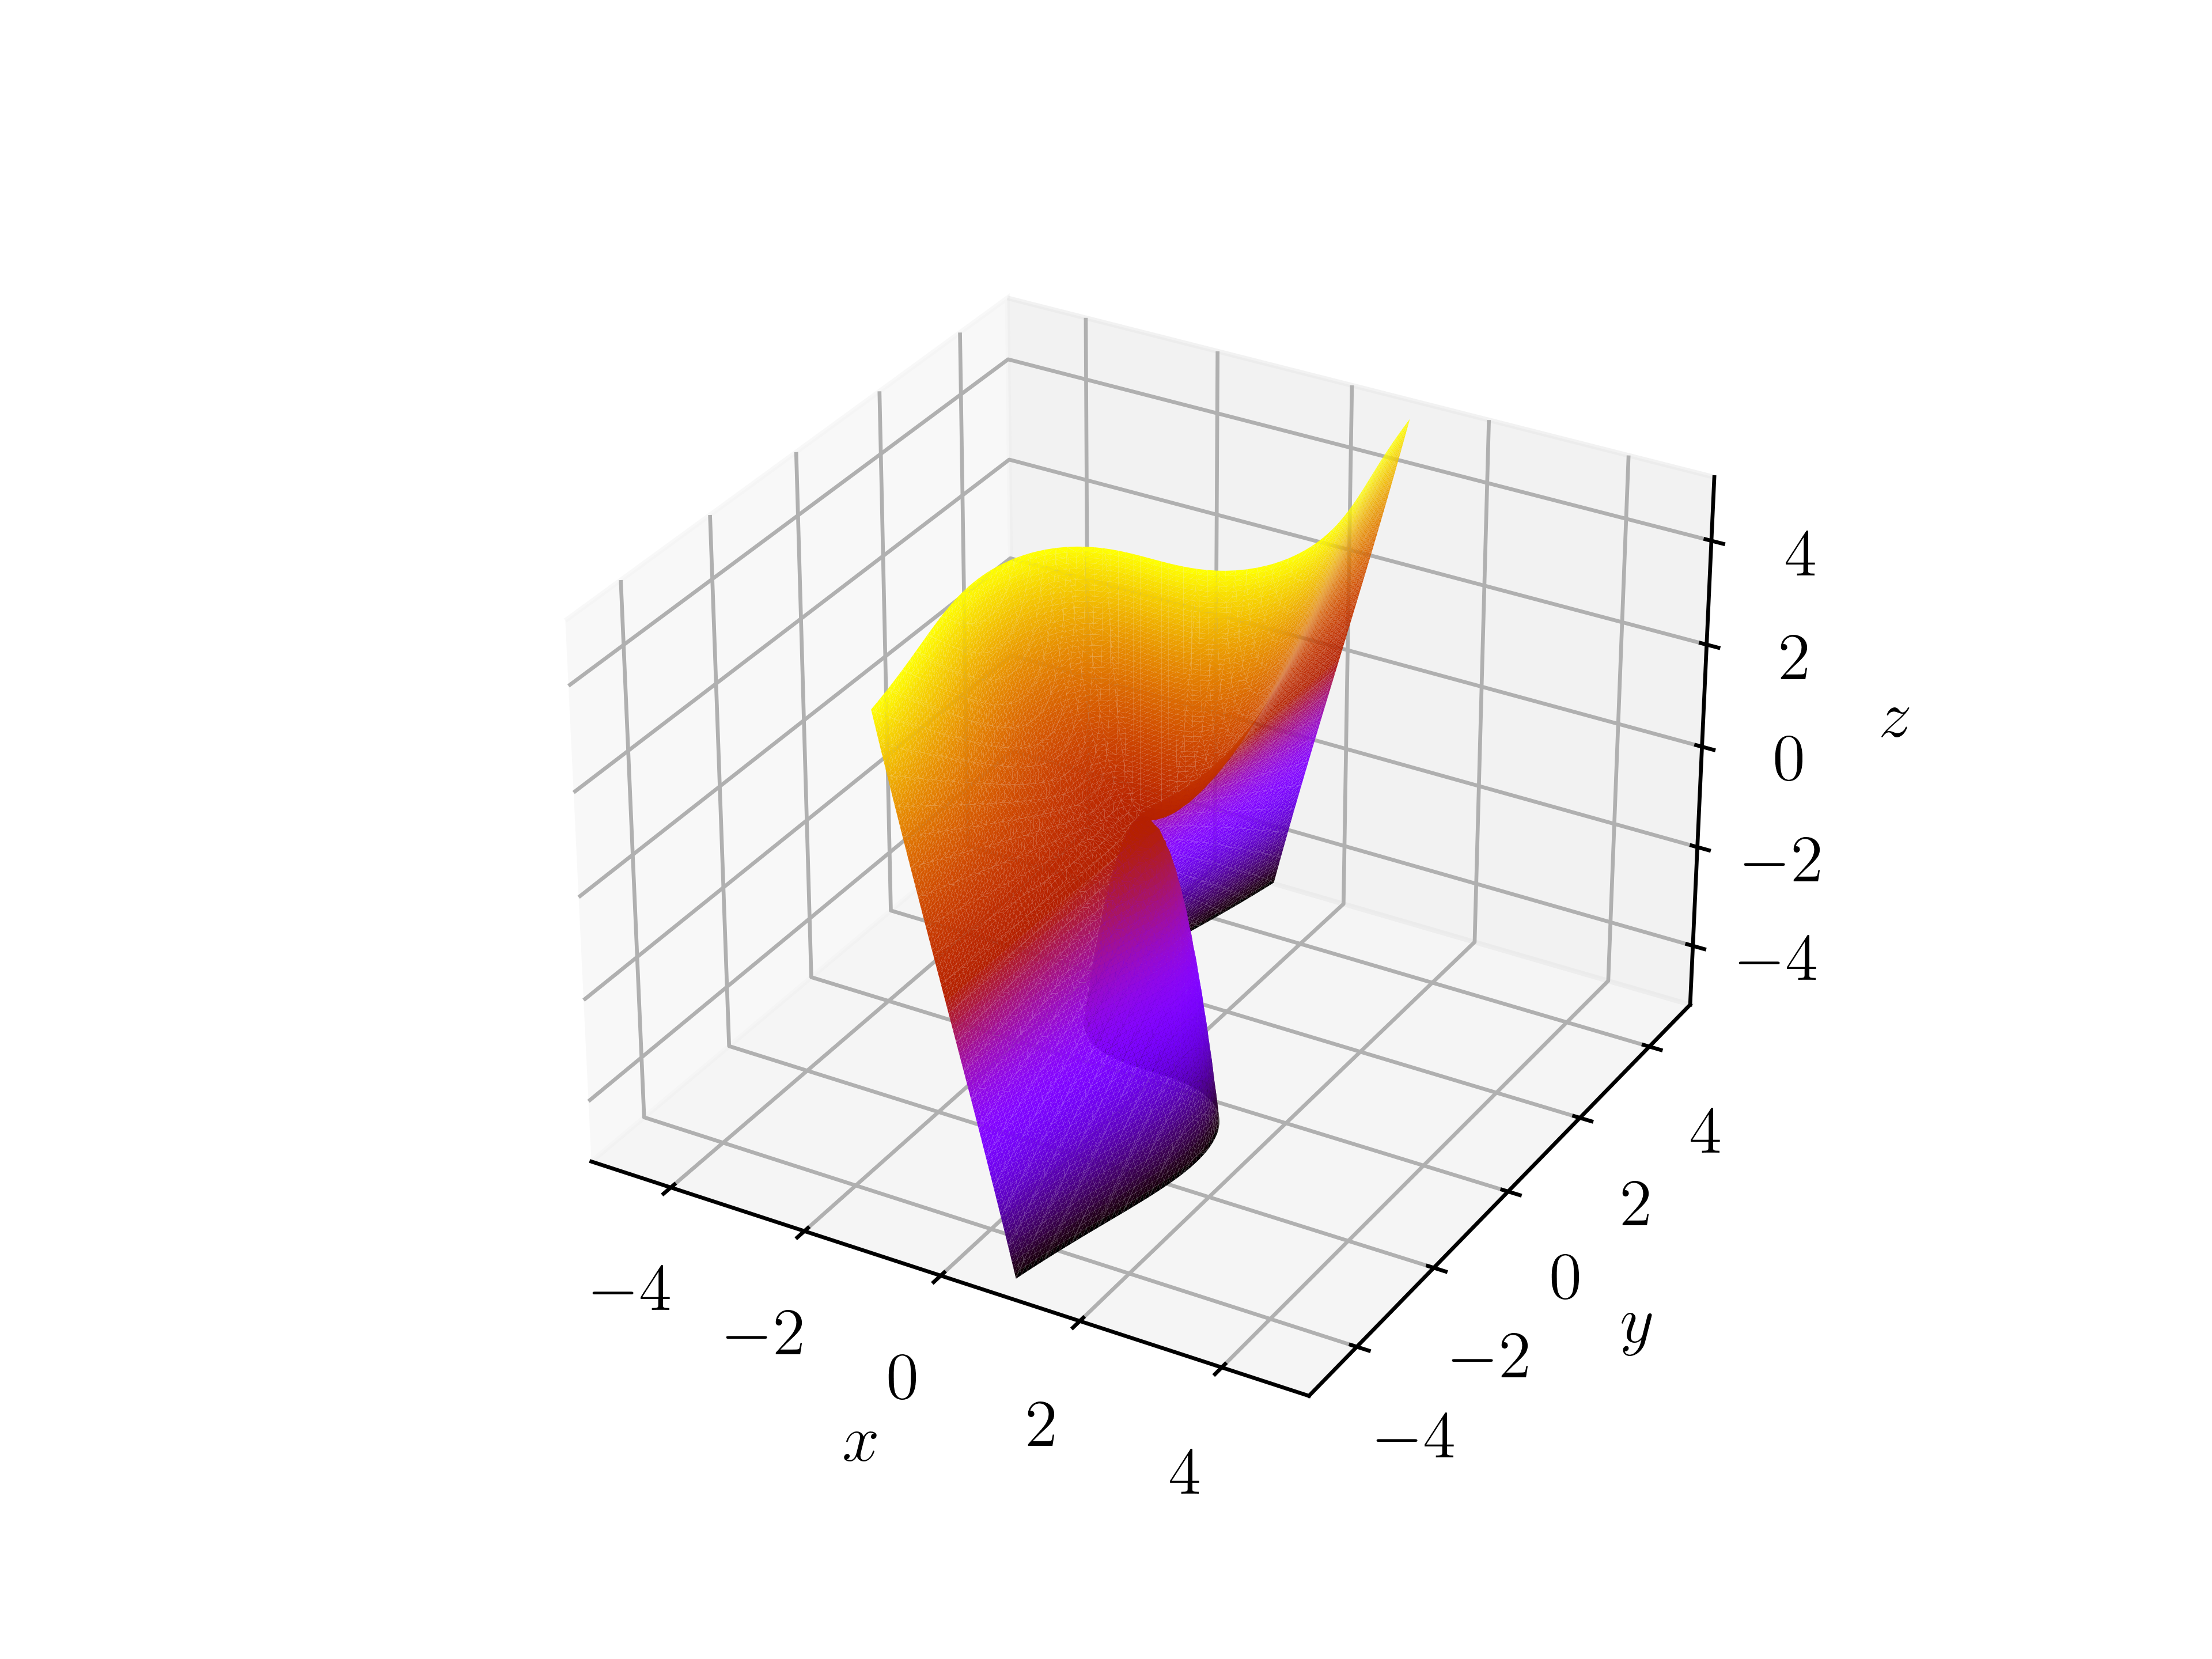
\includegraphics[scale=0.6]{./imagenes/Limite_No_Calculable_en_Polares.png}
      \vspace{-0.5cm}
      \caption{$f(x,y)=\dfrac{x^2y+y^3}{x}$}
    \end{figure}
  \end{center}
\end{frame}

\begin{frame}
  \begin{thm}
    Sea $U\subseteq\Real^n$ abierto, tal que $(0,0)$ es un punto de acumulación de $U$, $f:U\To\Real$, sea $F$ definida por
    $$F(r,\theta)=f(r\cos(\theta),r\sen(\theta))$$
    Si existe $H(r)$ tal que
    $$\abs{F(r,\theta)-L}\leq H(r),\ \forall\theta\in\Real$$
    y $\lim\limits_{r\to0}H(r)=0$, entonces
    $$\lim_{(x,y)\to(0,0)}f(x,y)=L$$
  \end{thm}
\end{frame}

\begin{frame}
  \begin{eg}
    Calcule el límite
    $$\lim_{(x,y)\to(0,0)}\dfrac{xy}{\sqrt{x^2+y^2}}$$
  \end{eg}
\end{frame}

%! subsección
\subsection{Continuidad}
\begin{frame}
\subsectionpage
\end{frame}

% \begin{frame}
% \tableofcontents[currentsubsection]
% \end{frame}

\begin{frame}{}
  \begin{defn}
    Sea $f:U\subseteq\Real^n\To\Real$ y $\vec{a}\in U$. Diremos que $f$ es \textbf{continua en $\vec{a}$} si y solo si
    $$\lim_{\vec{x}\to\vec{a}}f(\vec{x})=f(\vec{a})$$
  \end{defn}
\end{frame}

\begin{frame}
  \begin{eg}
    Demuestre que la función
    $$f(x,y)=\left\{\begin{array}{ll}
      \dfrac{x^2y}{x^2+y^2} & \text{si } (x,y)\neq(0,0)\\
      0 & \text{si } (x,y)=(0,0)
    \end{array}\right.$$
    es continua en $(0,0)$.
  \end{eg}
\end{frame}

\begin{frame}
  \begin{defn}
    Sea $f:U\subseteq\Real^n\To\Real$, diremos que $f$ es \textbf{continua en $U$} si y solo si $f$ es continua en todo punto de $U$.
  \end{defn}
\end{frame}

\begin{frame}
  \begin{eg}
    Sea $f:\Real^2\To\Real$ definida por
    $$f(x,y)=\left\{\begin{array}{ll}
      \dfrac{x^2y}{x^2+y^2} & \text{si } (x,y)\neq(0,0)\\
      0 & \text{si } (x,y)=(0,0)
    \end{array}\right.$$
    Encuentre los puntos de continuidad de $f$.
  \end{eg}
\end{frame}

\begin{frame}
  \begin{defn}
    Sea $F:U\subseteq\Real^n\To\Real^m$ y $\vec{a}\in U$. Diremos que $f$ es \textbf{continua en $\vec{a}$} si y solo si
    $$\lim_{\vec{x}\to\vec{a}}F(\vec{x})=f(\vec{a})$$
  \end{defn}
  \begin{thm}
    Sea $F:U\subseteq\Real^n\To\Real^m$ y $\vec{a}\in U$, si $F=(f_1,f_2,\ldots,f_m)$, entonces $F$ es continua en $\vec{a}$ si y solo si $f_i$ es continua en $\vec{a}$, $i=1,2,\ldots,m$.
  \end{thm}
\end{frame}

\begin{frame}
  \begin{eg}
    Demuestre que la función
    $$f(x,y)=(x^2y,x+y)$$
    es continua en $(0,0)$.
  \end{eg}
\end{frame}

\begin{frame}
  \begin{propo}
    Sean $f,g:U\subseteq\Real^n\To\Real$ funciones continuas, entonces
    \begin{enumerate}[<+->]
      \item $\alpha f+\beta g$ es continua
      \item $fg$ es continua
      \item Si $g(\vec{x})\neq0$, $\dfrac{f}{g}$ es continua
    \end{enumerate}
  \end{propo}
\end{frame}

\begin{frame}
  \begin{thm}
    Sean $f:U\subseteq\Real^n\To\Real^m$ y $g:V\subseteq\Real^m\To\Real^p$ funciones continuas, $f(U)\subseteq V$, entonces $g\circ f$ es continua.
  \end{thm}
\end{frame}

\begin{frame}
  \begin{eg}
    Analice la continuidad de la función
    $$f(x,y)=\left\{\begin{array}{ll}
      \sqrt{1-x^2-y^2} & \text{si } x^2+y^2\leq 1\\
      0 & \text{si } x^2+y^2>1
    \end{array}\right.$$
  \end{eg}
\end{frame}

%! subsección
\subsection{Ejercicios}
\begin{frame}
\subsectionpage
\end{frame}

% \begin{frame}
% \tableofcontents[currentsubsection]
% \end{frame}

\begin{frame}{Ejercicios}
  \begin{enumerate}
    \item Encuentre el límite o muestre que no existe\\[0.25cm]
    \begin{enumerate}
      \item $\displaystyle\lim_{(x,y)\to(3,5)}\ 3x^2y^2-2xy^3$
      \item $\displaystyle\lim_{(x,y)\to(3,\pi)}\ xy\cos\left(\dfrac{y}{x}\right)$
      \item $\displaystyle\lim_{(x,y)\to(1,2)}\dfrac{x^2+y^2}{x^2-y^2}$
      \item $\displaystyle\lim_{(x,y)\to(0,0)}\dfrac{x^2y^2}{x^2+y^2}$
      \item $\displaystyle\lim_{(x,y)\to(0,0)}\dfrac{x^2}{x^2+y^2}$
      \item $\displaystyle\lim_{(x,y)\to(0,0)}\dfrac{xy}{\sqrt{x^2+y^2}}$
      \item $\displaystyle\lim_{(x,y,z)\to(3,0,1)}\ e^{-xy}\cos(\pi z)$
      \item $\displaystyle\lim_{(x,y,z)\to(0,0,0)}\dfrac{x^2+2y^2+3z^2}{x^2+y^2+z^2}$
    \end{enumerate}
  \end{enumerate}
\end{frame}

\begin{frame}{Ejercicios}
  \begin{enumerate}
    \setcounter{enumi}{1}
    \item Analice la continuidad de las siguientes funciones\\[0.25cm]
    \begin{enumerate}
      \item $f(x,y)=\left\{\begin{array}{cl}
        \dfrac{x^3y^2}{x^2+y^2} & \text{si } (x,y)\neq(0,0)\\
        0 & \text{si } (x,y)=(0,0)
      \end{array}\right.$\\[0.25cm]
      \item $f(x,y)=\left\{\begin{array}{cl}
        \sqrt{1-x^2+y^2} & \text{si } x^2-y^2\leq 1\\
        0 & \text{si } x^2-y^2>1
      \end{array}\right.$
    \end{enumerate}
  \end{enumerate}
\end{frame}

\end{document}